% Provenance (never printed): see sources/outline_sources.md (Year 1: fault types and
% Anderson's theory; fold geometry and classification; foliation, schistosity and
% lineation; microstructures). Exercise and problem values in the Book 3 scratch calculator
% calc/ch17.py; the Varden Hills fold and fault from figdata/shared/region.py (read only).
% Fold, anticline, syncline and fold axis are owned by ch. 4; throw and heave by ch. 5;
% trend and plunge by ch. 6; the stresses and the Coulomb criterion by ch. 16. Shear zones
% and deformation mechanisms belong to the Year 3 volume (told here).
\chapter{Fallas, pliegues y fábricas}\label{ch:b1:faults-folds-fabrics}

Un corte de carretera muestra una cara de roca pulida como el vidrio y rayada por finos surcos paralelos. Al otro lado del valle,
un acantilado marino muestra capas de arenisca y lutita dobladas en zigzag, con lados rectos y esquinas agudas. En un tejado
cercano, unas pizarras se separan en láminas de unos pocos milímetros de espesor, según planos que cortan las capas del lodo
del que se formaron. Cada una es un registro de la deformación de la roca, leído a una escala distinta: los surcos dan la
dirección en la que dos bloques se deslizaron uno junto al otro a lo largo de una falla; los zigzags miden cuánto se
acortaron las capas; los planos de la pizarra crecieron atravesando el grano de la roca mientras se comprimía. Este capítulo
da la geometría necesaria para medir los tres registros, y la mecánica del capítulo anterior explica por qué las fallas
tienen los \omterm{def:b1:geological-maps:attitude}{buzamientos} que tienen.

\begin{recall}
La \omterm{def:b1:geological-maps:attitude}{actitud} de un plano es su \omterm{def:b1:geological-maps:attitude}{dirección de buzamiento} y su \omterm{def:b1:geological-maps:attitude}{buzamiento}, escritos por ejemplo como
$080/12$; su \omterm{def:b1:geological-maps:attitude}{rumbo} se obtiene por la regla de la mano derecha, con el plano buzando hacia la derecha de un observador que
mira a lo largo del \omterm{def:b1:geological-maps:attitude}{rumbo} (\cref{ch:b1:geological-maps}). Un \omterm{def:b1:geological-maps:fold}{pliegue} es una curvatura de capas originalmente planas; un
\omterm{def:b1:geological-maps:fold}{anticlinal} es convexo hacia arriba, con las rocas más antiguas en su núcleo, y un \omterm{def:b1:geological-maps:fold}{sinclinal} es cóncavo hacia arriba; el eje
del \omterm{def:b1:geological-maps:fold}{pliegue} es la línea a lo largo de la cual las capas se curvan más (\cref{ch:b1:geological-maps}). El salto y el \omterm{def:b1:cross-sections:throw}{salto
horizontal} de una falla son las componentes vertical y horizontal de su desplazamiento (\cref{ch:b1:cross-sections}). Una
recta tiene una tendencia y una \omterm{def:b1:field-lab-methods-1:trend-plunge}{inmersión}, y el vector unitario hacia abajo $(\cos p\sin t, \cos p\cos t, -\sin p)$
(\cref{ch:b1:field-lab-methods-1}). Una roca que obedece el criterio de Coulomb se rompe en planos a $\ang{45} - \phi/2$ de
$\sigma_1$, y las fallas existentes deslizan según la \omterm{prop:b1:stress-strain-rheology:byerlee}{ley de Byerlee} (\cref{ch:b1:stress-strain-rheology}). Un \omterm{def:b1:rock-forming-minerals:mineral}{mineral} está
en extinción entre polarizadores cruzados cuando sus direcciones de vibración son paralelas a las de los polarizadores
(\cref{ch:b1:optical-mineralogy}). Las fallas se estudiaron en el libro 1, año 7; las \omterm{def:b1:faults-folds-fabrics:fault-types}{fallas inversas}, los \omterm{def:b1:faults-folds-fabrics:fault-types}{cabalgamientos} y
la \omterm{def:b1:faults-folds-fabrics:foliation}{foliación}, en el libro 2, año 12. El producto vectorial de dos vectores es perpendicular a ambos (matemáticas, primer año
universitario).
\end{recall}

\section{Fallas: geometría y cinemática}\label{sec:b1:faults-folds-fabrics:faults}

Una falla es una superficie a lo largo de la cual dos bloques de roca se han desplazado uno junto al otro. Para describir el
movimiento necesitamos nombres para los dos bloques y para el desplazamiento, y una forma de medir su dirección dentro del
plano de la falla.

\begin{definition}[Bloque superior, bloque inferior, vector de deslizamiento, deslizamiento neto, cabeceo]\label{def:b1:faults-folds-fabrics:fault-elements}
Sea una falla localmente un plano que no es vertical. El \emph{bloque superior}\index{bloque superior} es el bloque situado
encima de ella, el \emph{bloque inferior}\index{bloque inferior} el situado debajo. Sea $A$ un punto del bloque inferior y $A'$
el punto del bloque superior que estaba en contacto con él antes del movimiento. El \emph{vector de deslizamiento}\index{vector de deslizamiento}
$\overrightarrow{AA'}$ es el desplazamiento del bloque superior respecto del bloque inferior; su longitud es el
\emph{deslizamiento neto}\index{deslizamiento neto}. El \emph{cabeceo}\index{cabeceo} $r$ (también llamado rake o pitch) del vector de deslizamiento es el ángulo, medido en el plano de la falla, desde la dirección del \omterm{def:b1:geological-maps:attitude}{rumbo} dada por
la regla de la mano derecha hasta el vector de deslizamiento, positivo cuando el vector apunta hacia arriba del plano y negativo
cuando apunta hacia abajo: $\ang{-180} < r \le \ang{180}$. Es la convención de los sismólogos, usada de nuevo para los
terremotos en \cref{ch:b1:earthquake-source}; muchos geólogos de campo anotan en cambio un ángulo entre 0 y \ang{180}, medido en
el sentido de las agujas del reloj desde el \omterm{def:b1:geological-maps:attitude}{rumbo} visto desde arriba, y añaden el sentido del movimiento con palabras.
\end{definition}
% ledger: ar:rake, ws:rake, ws:fault-terms

Los dos nombres vienen de la minería: un minero que trabajaba una veta inclinada se apoyaba en el \omterm{def:b1:faults-folds-fabrics:fault-elements}{bloque inferior} y tenía el
\omterm{def:b1:faults-folds-fabrics:fault-elements}{bloque superior} sobre la cabeza. Un desplazamiento visto en un solo corte no es, en general, el deslizamiento: una capa
desplazada en un mapa o en una sección muestra una separación, que depende de la \omterm{def:b1:geological-maps:attitude}{actitud} de la capa. El deslizamiento necesita
dos puntos que antes fueron uno, como las dos mitades de una línea cortada por la falla, por ejemplo el borde de un dique
frente a una capa.

\begin{omfigure}
\begin{tikzpicture}[>={Stealth[length=5pt]}, font=\small]
% (a) the fault plane seen face-on; slip vector of length 3.6 cm at rake -35 deg
% (normal and sinistral): strike-slip component 3.6 cos 35 = 2.949, dip-slip 3.6 sin 35 = 2.065
\pgfmathsetmacro{\Ls}{3.6*cos(35)}\pgfmathsetmacro{\Ld}{3.6*sin(35)}
\begin{scope}
  \fill[omDef!15] (0,0) rectangle (6.2,3.4);
  \draw[omDef, line width=0.7pt] (0,0) rectangle (6.2,3.4);
  \draw[line width=1.2pt] (0,3.4) -- (6.2,3.4);
  \node[anchor=south, font=\scriptsize] at (3.1,3.4) {línea de rumbo, donde la falla llega a la superficie};
  \draw[->, line width=0.6pt] (6.45,3.0) -- (6.45,2.0) node[midway, right, font=\scriptsize, align=left] {hacia abajo\\ por el buzamiento};
  \draw[->, line width=0.6pt] (0.3,0.35) -- (1.3,0.35) node[right, font=\scriptsize] {rumbo};
  \coordinate (A) at (1.2,2.55);
  \coordinate (B) at ($(A)+(\Ls,0)$);
  \coordinate (A2) at ($(A)+(\Ls,-\Ld)$);
  \draw[omProp, dashed, line width=0.7pt] (A) -- (B) node[midway, above, font=\scriptsize] {componente de rumbo};
  \draw[omProp, dashed, line width=0.7pt] (B) -- (A2) node[midway, right, font=\scriptsize, align=left] {componente\\ de buzamiento};
  \draw[->, line width=1.3pt, omThm] (A) -- (A2) node[midway, below left, font=\scriptsize, inner sep=1pt] {vector de deslizamiento};
  \draw[black] ($(A)+(0.9,0)$) arc[start angle=0, end angle=-35, radius=0.9];
  \node[font=\scriptsize] at ($(A)+(-17.5:1.15)$) {$r$};
  \fill (A) circle[radius=1.4pt] node[above left, inner sep=1.5pt] {$A$};
  \fill (A2) circle[radius=1.4pt] node[below right, inner sep=1.5pt] {$A'$};
  \node[font=\small\bfseries] at (3.1,-0.55) {(a) en el plano de la falla};
\end{scope}
% (b) the vertical section through the dip line: dip 50 deg; dip-slip 2.065 -> throw 1.582, heave 1.327
\begin{scope}[xshift=9.4cm, yshift=0.2cm]
  \pgfmathsetmacro{\th}{\Ld*sin(50)}\pgfmathsetmacro{\he}{\Ld*cos(50)}
  \fill[omLithSand!40] (-1.2,0) -- (-1.2,3.2) -- (0,3.2) -- ({3.2/tan(50)},0) -- cycle;
  \fill[omLithSand!20] ({3.2/tan(50)},0) -- (0,3.2) -- (4.2,3.2) -- (4.2,0) -- cycle;
  \draw[line width=0.6pt] (-1.2,3.2) -- (4.2,3.2);
  \draw[omDef, line width=1.1pt] (0,3.2) -- ({3.2/tan(50)},0);
  \draw[black] (0.75,3.2) arc[start angle=0, end angle=-50, radius=0.75];
  \node[font=\scriptsize] at ($(0,3.2)+(-25:1.0)$) {$\delta$};
  \coordinate (P) at ({1.3*cos(50)},{3.2-1.3*sin(50)});
  \coordinate (Q) at ($(P)+({\Ld*cos(50)},{-\Ld*sin(50)})$);
  \coordinate (R) at ($(P)+(\he,0)$);
  \draw[->, omProp, line width=1.1pt] (P) -- (Q);
  \draw[black!80, densely dotted, line width=0.7pt] (P) -- (R) node[midway, above, font=\scriptsize] {salto horizontal};
  \draw[black!80, densely dotted, line width=0.7pt] (R) -- (Q) node[midway, right, font=\scriptsize] {salto};
  \node[font=\scriptsize, omProp, anchor=east] at ($(P)!0.55!(Q)+(-0.08,0)$) {deslizamiento de buzamiento};
  \node[font=\small] at (3.3,2.6) {bloque superior};
  \node[font=\small] at (-0.55,1.0) {bloque inferior};
  \node[font=\small\bfseries] at (1.5,-0.75) {(b) en el plano vertical del buzamiento};
\end{scope}
\end{tikzpicture}
\par\smallskip{\small El elemento de una falla, dibujado a escala para una falla de \omterm{def:b1:geological-maps:attitude}{buzamiento} $\delta = \ang{50}$ y un \omterm{def:b1:faults-folds-fabrics:fault-elements}{vector de
deslizamiento} de \omterm{def:b1:faults-folds-fabrics:fault-elements}{cabeceo} $r = \ang{-35}$. (a) El plano de la falla visto de frente: el \omterm{def:b1:faults-folds-fabrics:fault-elements}{vector de deslizamiento}
$\overrightarrow{AA'}$ se descompone en una componente según el \omterm{def:b1:geological-maps:attitude}{rumbo} y otra según el \omterm{def:b1:geological-maps:attitude}{buzamiento}. (b) La sección vertical
perpendicular al \omterm{def:b1:geological-maps:attitude}{rumbo}: la componente de deslizamiento de \omterm{def:b1:geological-maps:attitude}{buzamiento} se descompone en el salto y el \omterm{def:b1:cross-sections:throw}{salto horizontal}.}
\label{fig:b1:faults-folds-fabrics:elements}
\end{omfigure}

\begin{proposition}[Componentes del deslizamiento]\label{prop:b1:faults-folds-fabrics:slip-components}
Sea una falla de \omterm{def:b1:geological-maps:attitude}{dirección de buzamiento} $\alpha$ y \omterm{def:b1:geological-maps:attitude}{buzamiento} $\delta$, y un \omterm{def:b1:faults-folds-fabrics:fault-elements}{vector de deslizamiento} de
longitud $L$ y \omterm{def:b1:faults-folds-fabrics:fault-elements}{cabeceo} $r$. Con componentes hacia el este, el norte y arriba, sean
$\mathbf s = (\sin(\alpha-\ang{90}), \cos(\alpha-\ang{90}), 0)$ el vector unitario según el \omterm{def:b1:geological-maps:attitude}{rumbo} y
$\mathbf u = (-\cos\delta\sin\alpha,
-\cos\delta\cos\alpha, \sin\delta)$ el vector unitario hacia arriba según el \omterm{def:b1:geological-maps:attitude}{buzamiento}. Entonces
\[
  \overrightarrow{AA'} = L\,(\cos r\,\mathbf s + \sin r\,\mathbf u),
\]
su componente de deslizamiento de \omterm{def:b1:geological-maps:attitude}{rumbo} es $L\cos r$ y su componente de deslizamiento de \omterm{def:b1:geological-maps:attitude}{buzamiento} $L\sin r$;
el salto es $L\,|\sin r|\sin\delta$, el \omterm{def:b1:cross-sections:throw}{salto horizontal} $L\,|\sin r|\cos\delta$, y el \omterm{def:b1:faults-folds-fabrics:fault-elements}{vector de
deslizamiento} tiene una \omterm{def:b1:field-lab-methods-1:trend-plunge}{inmersión} $p$, con $\sin p = |\sin r|\sin\delta$.
\end{proposition}

\begin{proof}
El vector $\mathbf s$ es horizontal y apunta según el \omterm{def:b1:geological-maps:attitude}{rumbo}; $\mathbf u$ es lo opuesto al vector unitario hacia abajo de la
línea de \omterm{def:b1:geological-maps:attitude}{buzamiento}, que tiene tendencia $\alpha$ e \omterm{def:b1:field-lab-methods-1:trend-plunge}{inmersión} $\delta$ (\cref{ch:b1:field-lab-methods-1}). Ambos están en el
plano de la falla, y $\mathbf s\cdot\mathbf u = -\cos\delta(\sin(\alpha -
\ang{90})\sin\alpha + \cos(\alpha - \ang{90})\cos\alpha) = -\cos\delta\cos\ang{90} = 0$,
así que forman una base ortonormal del plano. Un vector del plano de longitud $L$ que forma el ángulo $r$ con $\mathbf s$,
contado hacia $\mathbf u$, es $L(\cos r\,\mathbf s + \sin r\,\mathbf u)$. Su componente vertical es
$L\sin r\sin\delta$, cuyo tamaño es el salto; su parte horizontal transversal al \omterm{def:b1:geological-maps:attitude}{rumbo} es $L\sin r$ por la parte horizontal de
$\mathbf u$, de longitud $\cos\delta$, que es el \omterm{def:b1:cross-sections:throw}{salto horizontal}; y el seno de su \omterm{def:b1:field-lab-methods-1:trend-plunge}{inmersión} es su componente vertical
dividida por $L$.
\end{proof}

En una falla de deslizamiento de \omterm{def:b1:geological-maps:attitude}{buzamiento}, $|\sin r| = 1$ y el \omterm{def:b1:cross-sections:throw}{salto horizontal} es el salto dividido por
$\tan\delta$, como en \cref{ch:b1:cross-sections}. El \omterm{def:b1:faults-folds-fabrics:fault-elements}{cabeceo} clasifica las fallas en familias.

\begin{definition}[Fallas normales, inversas, cabalgamientos, de desgarre y oblicuas]\label{def:b1:faults-folds-fabrics:fault-types}
Una falla cuyo \omterm{def:b1:faults-folds-fabrics:fault-elements}{vector de deslizamiento} yace según la línea de \omterm{def:b1:geological-maps:attitude}{buzamiento} ($r = \pm\ang{90}$) es una falla de deslizamiento de
\omterm{def:b1:geological-maps:attitude}{buzamiento}: una \emph{falla normal}\index{falla normal} cuando el \omterm{def:b1:faults-folds-fabrics:fault-elements}{bloque superior} ha bajado ($r = \ang{-90}$), una
\emph{falla inversa}\index{falla inversa} cuando ha subido ($r = \ang{90}$). Un \emph{cabalgamiento}\index{cabalgamiento} es una
falla inversa que buza \ang{45} o menos. Una falla cuyo deslizamiento es paralelo a su \omterm{def:b1:geological-maps:attitude}{rumbo} ($r = 0$ o \ang{180}) es una
\emph{falla de desgarre}\index{falla de desgarre}; estas fallas suelen ser casi verticales. Una falla de desgarre es
\emph{dextral}\index{dextral} (lateral derecha) cuando un observador de pie a un lado ve el otro lado desplazado a la derecha,
y \emph{sinistral}\index{sinistral} (lateral izquierda) cuando a la izquierda. Una falla cuyo deslizamiento tiene a la vez una
componente de desgarre y una de \omterm{def:b1:geological-maps:attitude}{buzamiento} es una \emph{falla oblicua}\index{falla oblicua}; en la práctica una falla se nombra
según su componente mayor, de modo que un \omterm{def:b1:faults-folds-fabrics:fault-elements}{cabeceo} cercano a \ang{-90} se llama normal.
\end{definition}
% ledger: usgs:fault-types, ws:fault-terms, ar:rake

\begin{proposition}[El sentido de una falla de desgarre]\label{prop:b1:faults-folds-fabrics:sense}
El sentido de una \omterm{def:b1:faults-folds-fabrics:fault-types}{falla de desgarre} no depende del lado en el que se sitúe el observador. Un \omterm{def:b1:faults-folds-fabrics:fault-elements}{cabeceo} cercano a $0$ es
\omterm{def:b1:faults-folds-fabrics:fault-types}{sinistral}, uno cercano a \ang{180} \omterm{def:b1:faults-folds-fabrics:fault-types}{dextral}.
\end{proposition}

\begin{proof}
Si un observador en el bloque 1 ve que el bloque 2 se mueve según $\mathbf v$, un observador en el bloque 2 ve que el bloque 1
se mueve según $-\mathbf v$. Al volverse para mirar al bloque 1, el segundo observador ha intercambiado izquierda y derecha.
Los dos cambios se cancelan: ambos ven el otro lado moverse en el mismo sentido, a la derecha o a la izquierda. Para la
segunda parte, colóquese sobre el \omterm{def:b1:faults-folds-fabrics:fault-elements}{bloque inferior} y mire al \omterm{def:b1:faults-folds-fabrics:fault-elements}{bloque superior}: entonces se mira según la \omterm{def:b1:geological-maps:attitude}{dirección de
buzamiento}, y como el plano buza a la derecha de su \omterm{def:b1:geological-maps:attitude}{rumbo}, la dirección del \omterm{def:b1:geological-maps:attitude}{rumbo} apunta a la izquierda. Un \omterm{def:b1:faults-folds-fabrics:fault-elements}{cabeceo} de $0$
mueve el \omterm{def:b1:faults-folds-fabrics:fault-elements}{bloque superior} según el \omterm{def:b1:geological-maps:attitude}{rumbo}, hacia la izquierda; un \omterm{def:b1:faults-folds-fabrics:fault-elements}{cabeceo} de \ang{180}, hacia la derecha.
\end{proof}

Una superficie de falla suele ser en sí misma un registro del movimiento: los rayados y las fibras sobre ella yacen a lo largo
del deslizamiento. Alrededor de la superficie, una zona de falla puede estar rellena de roca rota por el movimiento.

\begin{definition}[Espejo de falla, estrías de falla, rocas de falla]\label{def:b1:faults-folds-fabrics:fault-rocks}
Las \emph{estrías de falla}\index{estrías de falla} son rayados o fibras sobre una superficie de falla, paralelos al
deslizamiento; un \emph{espejo de falla}\index{espejo de falla} es una superficie de falla que las lleva, a menudo alisada por
el deslizamiento. Una \emph{roca de falla}\index{roca de falla} es una roca producida por el movimiento en una falla. Una
\emph{brecha de falla}\index{brecha de falla} está formada por fragmentos angulosos de las paredes de la falla, rotados y
desplazados de su sitio, desde bloques enormes hasta unos \qty{2}{mm}; una \emph{cataclasita}\index{cataclasita} está formada
por fragmentos del tamaño de la arena o menores; ninguna tiene fábrica, pues los fragmentos yacen al azar. Una
\emph{arcilla de falla}\index{arcilla de falla} es una roca de falla rica en arcilla, muy blanda en el afloramiento. Una
\emph{milonita}\index{milonita} es una roca de grano fino y muy foliada, producida en una zona de cizalla por cizalla dúctil,
con los granos reducidos por recristalización más que por trituración.
\end{definition}
% ledger: ws:fault-terms, ws:fault-rocks

Las \omterm{def:b1:faults-folds-fabrics:fault-rocks}{rocas de falla} son un calibre de profundidad, y siguen la \omterm{def:b1:stress-strain-rheology:strength-envelope}{envolvente de resistencia} de
\cref{ch:b1:stress-strain-rheology}. La \omterm{def:b1:faults-folds-fabrics:fault-rocks}{arcilla de falla}, la brecha y la \omterm{def:b1:faults-folds-fabrics:fault-rocks}{cataclasita}, con su fábrica al azar, se producen por
deslizamiento friccional y fractura en la \omterm{def:b1:layered-earth:layers}{corteza} frágil; las \omterm{def:b1:faults-folds-fabrics:fault-rocks}{milonitas} se producen por debajo de la \omterm{def:b1:stress-strain-rheology:strength-envelope}{transición frágil--dúctil},
donde la falla continúa hacia abajo como una banda de cizalla dúctil. Para un geoterma normal y agua suficiente, la transición
entre ambas se sitúa a \qtyrange{10}{15}{km}, cerca de los \qty{13.7}{km} de la envolvente del capítulo anterior, y la falla es
más fuerte allí. En una gran falla traída desde profundidad se encuentra, lado a lado, el mismo orden: zonas de \omterm{def:b1:faults-folds-fabrics:fault-rocks}{arcilla de
falla} cerca de la superficie, luego \omterm{def:b1:faults-folds-fabrics:fault-rocks}{cataclasita}, y luego \omterm{def:b1:faults-folds-fabrics:fault-rocks}{milonita}.
El nombre \omterm{def:b1:faults-folds-fabrics:fault-rocks}{milonita}, de la palabra griega para moler harina, recoge un error: se creyó que era roca molida. El volumen del año 3
estudia esas zonas de cizalla profundas y los mecanismos que forman las \omterm{def:b1:faults-folds-fabrics:fault-rocks}{milonitas}.
% ledger: sibson:fault-rocks, sibson:alpine-fault, ws:fault-rocks

\begin{omfigure}
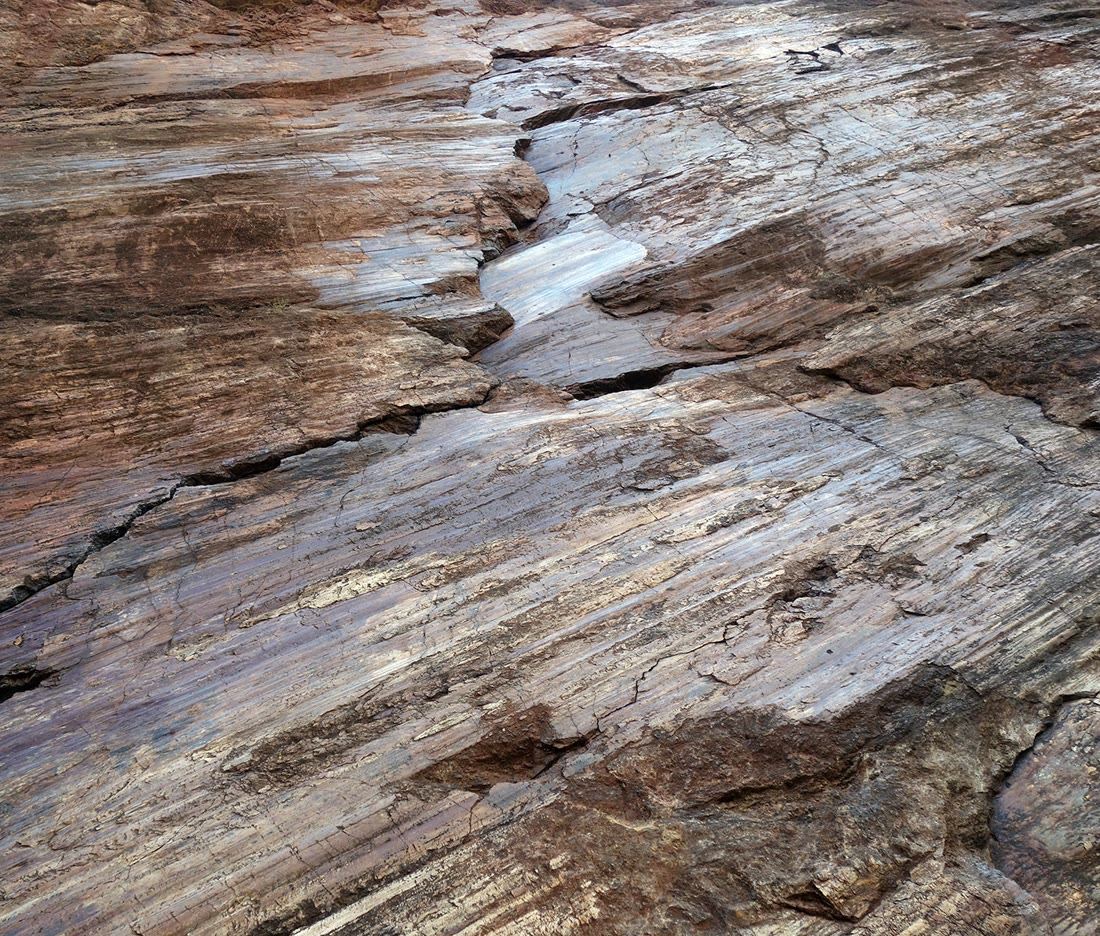
\includegraphics[height=5.2cm]{images/book3/b1-slickenside.jpg}\hfill
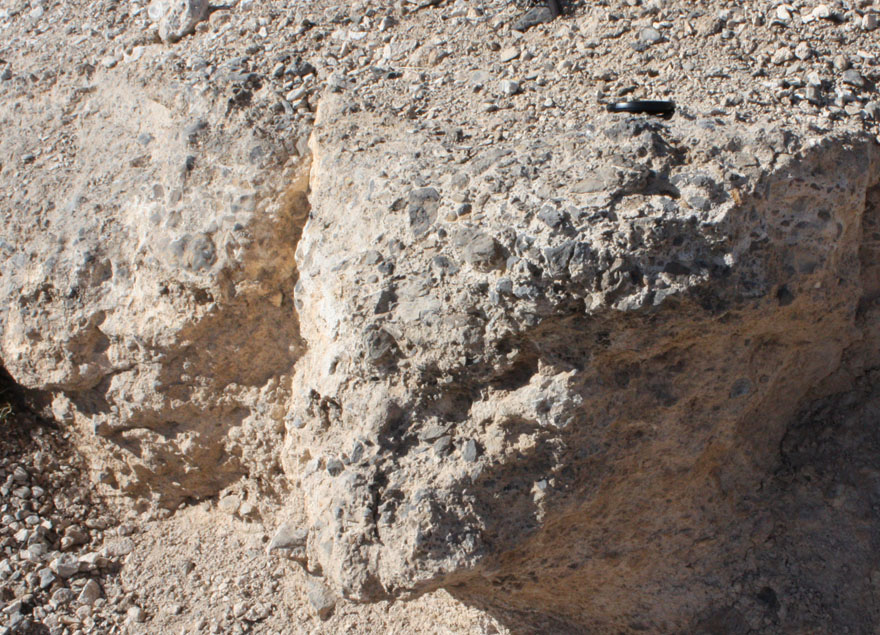
\includegraphics[height=5.2cm]{images/book3/b1-fault-breccia.jpg}
\par\smallskip{\small Izquierda: un \omterm{def:b1:faults-folds-fabrics:fault-rocks}{espejo de falla} en sílex, de unos \qtyproduct{3 x 3}{m} de una superficie de \qty{10}{m} de altura,
Corona Heights, San Francisco; la cara pulida está estriada según el deslizamiento. Fotografía: Dextersinister, CC~BY-SA~4.0.
Derecha: \omterm{def:b1:faults-folds-fabrics:fault-rocks}{brecha de falla} del \omterm{def:b1:faults-folds-fabrics:fault-types}{cabalgamiento} Keystone, Red Rock Canyon, Nevada: fragmentos angulosos de roca carbonatada gris en
una matriz más clara; la tapa de objetivo en la esquina superior derecha mide \qty{5.8}{cm} de diámetro. Fotografía: Jstuby,
dominio público. Ambas de Wikimedia Commons.}
\label{fig:b1:faults-folds-fabrics:fault-surfaces}
\end{omfigure}
% ledger: commons:slickenside, commons:breccia

\begin{method}[Medición del deslizamiento en una falla]\label{met:b1:faults-folds-fabrics:slip}
\begin{enumerate}
  \item Mídase la \omterm{def:b1:geological-maps:attitude}{actitud} $\alpha/\delta$ de la superficie de falla y escríbase su \omterm{def:b1:geological-maps:attitude}{rumbo}, $\alpha - \ang{90}$.
  \item Mídanse las estrías: su \omterm{def:b1:faults-folds-fabrics:fault-elements}{cabeceo} sobre la falla, o su tendencia e \omterm{def:b1:field-lab-methods-1:trend-plunge}{inmersión}; para un \omterm{def:b1:faults-folds-fabrics:fault-elements}{cabeceo} $r$, $\sin p = |\sin r|\sin\delta$.
  \item Averígüese en qué sentido se movió el \omterm{def:b1:faults-folds-fabrics:fault-elements}{bloque superior}, a partir de marcadores desplazados a través de la falla, y
        dése al \omterm{def:b1:faults-folds-fabrics:fault-elements}{cabeceo} su signo: negativo si el \omterm{def:b1:faults-folds-fabrics:fault-elements}{bloque superior} bajó.
  \item Hállese el \omterm{def:b1:faults-folds-fabrics:fault-elements}{deslizamiento neto} $L$ a partir de dos puntos que antes fueron uno; si solo se conoce el salto $h$ de un
        marcador horizontal, $L = h/(|\sin r|\sin\delta)$.
  \item Calcúlense las componentes con
        \cref{prop:b1:faults-folds-fabrics:slip-components} y nómbrese la falla
        con \cref{def:b1:faults-folds-fabrics:fault-types}.
\end{enumerate}
\end{method}

\begin{inthefield}[Medición de una superficie de falla]
Un geólogo que encuentra una superficie de falla en un afloramiento la mide como cualquier otro plano, con una brújula
clinómetro apoyada sobre la superficie, y luego mide las \omterm{def:b1:faults-folds-fabrics:fault-rocks}{estrías de falla} sobre ella, bien como \omterm{def:b1:faults-folds-fabrics:fault-elements}{cabeceo}, con un transportador
apoyado sobre el plano, bien como tendencia e \omterm{def:b1:field-lab-methods-1:trend-plunge}{inmersión}. Las dos medidas se comprueban entre sí con la fórmula del paso~2 del
método. El sentido del movimiento es la parte difícil. Los pequeños escalones sobre un \omterm{def:b1:faults-folds-fabrics:fault-rocks}{espejo de falla}, y las fibras de cuarzo
o calcita que crecieron mientras los bloques se separaban, pueden mostrar hacia dónde se fue el bloque que falta, pero algunos
escalones apuntan en sentido contrario, así que el sentido solo se da por bueno cuando concuerda con el desplazamiento de una
capa marcadora o de una veta. Las \omterm{def:b1:faults-folds-fabrics:fault-rocks}{rocas de falla} se describen y se muestrean, y una zona de falla demasiado ancha para medirla
en un solo lugar se cartografía como una banda. Cada falla se anota en una estación numerada del cuaderno, con su \omterm{def:b1:geological-maps:attitude}{actitud}, sus
estrías, el sentido del movimiento y lo seguro que está el geólogo de él.
\end{inthefield}

\section{La teoría de Anderson del fallamiento}\label{sec:b1:faults-folds-fabrics:anderson}

¿Por qué son empinadas la mayoría de las \omterm{def:b1:faults-folds-fabrics:fault-types}{fallas normales} y suaves la mayoría de los \omterm{def:b1:faults-folds-fabrics:fault-types}{cabalgamientos}? En 1905 el geólogo
escocés Ernest Masson Anderson respondió con dos observaciones: la superficie de la Tierra fija las direcciones de los
\omterm{def:b1:stress-strain-rheology:principal}{esfuerzos principales}, y el criterio de Coulomb fija entonces el ángulo de las fallas.
% ledger: ws:anderson, anderson:1905

\begin{proposition}[Una superficie libre es un plano principal]\label{prop:b1:faults-folds-fabrics:free-surface}
En la superficie de la Tierra, donde es horizontal, uno de los \omterm{def:b1:stress-strain-rheology:principal}{esfuerzos principales} es vertical y los otros dos son
horizontales.
\end{proposition}

\begin{proof}
El aire presiona el suelo solo con su presión, normal a la superficie: no ejerce esfuerzo de cizalla. El esfuerzo sobre el plano
horizontal de la superficie es, por tanto, normal a él. En tres dimensiones, el esfuerzo sobre un plano de normal unitaria
$\mathbf n$ es el vector $\boldsymbol\sigma\mathbf n$ (libros de física, año 3); si no tiene parte de cizalla, es paralelo a
$\mathbf n$, de modo que $\boldsymbol\sigma\mathbf n = \lambda\mathbf n$ y $\mathbf n$ es un vector propio de la matriz
simétrica $\boldsymbol\sigma$: una dirección principal (\cref{def:b1:stress-strain-rheology:principal}). La vertical es así
una dirección principal, y las otras dos, perpendiculares a ella, son horizontales.
\end{proof}

Anderson supuso que los \omterm{def:b1:stress-strain-rheology:principal}{esfuerzos principales} conservan estas direcciones hasta las profundidades a las que se forman las
fallas. La suposición se cumple bien bajo una superficie de poca pendiente y en rocas sin debilidades antiguas fuertes; falla
cerca de un relieve empinado y donde fallas o capas antiguas guían las nuevas. Con ella, solo son posibles tres casos, según
cuál de $\sigma_1$, $\sigma_2$ y $\sigma_3$ sea vertical.

\begin{theorem}[Teoría de Anderson del fallamiento]\label{thm:b1:faults-folds-fabrics:anderson}
Sea un esfuerzo principal vertical y sea la roca la que se rompe según el criterio de Coulomb, con \omterm{def:b1:stress-strain-rheology:coulomb}{ángulo de fricción interna}
$\phi$. Las fallas nuevas se forman en planos que contienen la dirección de $\sigma_2$ y forman el ángulo $\ang{45} - \phi/2$
con $\sigma_1$, y deslizan perpendicularmente a $\sigma_2$, acortando la roca según $\sigma_1$. Por tanto:
\begin{enumerate}[label=(\alph*)]
  \item si $\sigma_1$ es vertical, se forman \omterm{def:b1:faults-folds-fabrics:fault-types}{fallas normales}, con \omterm{def:b1:geological-maps:attitude}{rumbo} según $\sigma_2$ y \omterm{def:b1:geological-maps:attitude}{buzamiento}
        $\ang{45} + \phi/2$;
  \item si $\sigma_3$ es vertical, se forman \omterm{def:b1:faults-folds-fabrics:fault-types}{cabalgamientos}, con \omterm{def:b1:geological-maps:attitude}{rumbo} según $\sigma_2$ y \omterm{def:b1:geological-maps:attitude}{buzamiento}
        $\ang{45} - \phi/2$;
  \item si $\sigma_2$ es vertical, se forman \omterm{def:b1:faults-folds-fabrics:fault-types}{fallas de desgarre} verticales, con \omterm{def:b1:geological-maps:attitude}{rumbo} a
        $\ang{45} - \phi/2$ a ambos lados de $\sigma_1$.
\end{enumerate}
Con $\phi = \ang{30}$, los \omterm{def:b1:geological-maps:attitude}{buzamientos} son \ang{60}, \ang{30} y \ang{90}.
\end{theorem}
\index{teoría de Anderson del fallamiento}

\begin{proof}
En un plano que contiene la dirección de $\sigma_2$, la normal yace en el plano de $\sigma_1$ y $\sigma_3$, y el esfuerzo sobre
el plano es el del problema bidimensional de \cref{ch:b1:stress-strain-rheology}: su punto yace sobre el círculo de Mohr de
$\sigma_1$ y $\sigma_3$, y su parte de cizalla yace en el plano de $\sigma_1$ y $\sigma_3$, perpendicular a $\sigma_2$. En
cualquier otro plano, el punto $(\sigma_n, \tau)$ queda dentro de ese círculo, que es el mayor de los tres círculos de Mohr de
un estado de esfuerzos tridimensional (admitido de la teoría tridimensional). Al crecer los esfuerzos, la recta de Coulomb es
por tanto tocada primero por los planos que contienen $\sigma_2$, y entre ellos, por \cref{thm:b1:stress-strain-rheology:failure-angle},
por los que están a $\ang{45} - \phi/2$ de $\sigma_1$. El deslizamiento sobre tal plano, perpendicular a $\sigma_2$, acerca los
dos bloques a lo largo de la dirección de mayor compresión y los separa a lo largo de la menor, como debe ser para aliviar el
esfuerzo. En el caso (a) el plano forma con la vertical el ángulo $\ang{45} - \phi/2$, así que buza $\ang{45} + \phi/2$; tiene
\omterm{def:b1:geological-maps:attitude}{rumbo} según la horizontal $\sigma_2$; el deslizamiento yace en el plano vertical del \omterm{def:b1:geological-maps:attitude}{buzamiento}, y el \omterm{def:b1:faults-folds-fabrics:fault-elements}{bloque superior} baja,
alargando la roca horizontalmente: una \omterm{def:b1:faults-folds-fabrics:fault-types}{falla normal}. En el caso (b) el plano forma $\ang{45} - \phi/2 < \ang{45}$ con la
horizontal $\sigma_1$, y el deslizamiento acorta la roca horizontalmente, empujando el \omterm{def:b1:faults-folds-fabrics:fault-elements}{bloque superior} hacia arriba: un
\omterm{def:b1:faults-folds-fabrics:fault-types}{cabalgamiento}. En el caso (c) los planos contienen la vertical, así que son verticales; el deslizamiento es horizontal,
perpendicular a $\sigma_2$: \omterm{def:b1:faults-folds-fabrics:fault-types}{fallas de desgarre}, a $\ang{45} - \phi/2$ a ambos lados de la horizontal $\sigma_1$.
\end{proof}

En cada régimen son posibles dos conjuntos de fallas, simétricos respecto de $\sigma_1$: fallas conjugadas, que se cortan con
un ángulo de $\ang{90} - \phi$, unos \ang{60}, con $\sigma_1$ en el ángulo agudo entre ellas. A la inversa, un par de fallas
conjugadas medido en el campo da las direcciones de los esfuerzos que las formaron: $\sigma_1$ biseca su ángulo agudo, y
$\sigma_2$ es su línea de intersección.

\begin{omfigure}
\begin{tikzpicture}[x={(1cm,0cm)}, y={(0.42cm,0.30cm)}, z={(0cm,1cm)},
  >={Stealth[length=5pt]}, font=\small, scale=0.86,
  face/.style={draw=black, line width=0.5pt, line join=round},
  sone/.style={->, line width=1.6pt, omThm},
  sthree/.style={->, line width=0.8pt, omDef}]
% exact geometry: the fault plane is X = xf(Z); slip is along the dip; throw t
% (a) normal fault: dip 60, xf(Z) = 1.3 + (1.6 - Z)/tan 60, throw 0.45
\begin{scope}
  \def\W{3.2}\def\D{1.6}\def\H{1.6}
  \pgfmathsetmacro{\c}{1/tan(60)}
  \pgfmathsetmacro{\xa}{1.3+1.6*\c}       % xf(0)
  \pgfmathsetmacro{\xb}{1.3+0.45*\c}      % xf(H - t)
  \pgfmathsetmacro{\mfa}{1.3+(1.6-0.55)*\c}\pgfmathsetmacro{\mfb}{1.3+(1.6-0.85)*\c}
  \pgfmathsetmacro{\mha}{1.3+(1.6-0.10)*\c}\pgfmathsetmacro{\mhb}{1.3+(1.6-0.40)*\c}
  % footwall
  \fill[omLithSand!55] (0,0,0) -- (\xa,0,0) -- (1.3,0,\H) -- (0,0,\H) -- cycle;
  \fill[omProp!40] (0,0,0.55) -- (\mfa,0,0.55) -- (\mfb,0,0.85) -- (0,0,0.85) -- cycle;
  \draw[face] (0,0,0) -- (\xa,0,0) -- (1.3,0,\H) -- (0,0,\H) -- cycle;
  \draw[face, fill=omLithSand!35] (0,0,\H) -- (1.3,0,\H) -- (1.3,\D,\H) -- (0,\D,\H) -- cycle;
  \draw[face, fill=black!12] (1.3,0,\H) -- (\xb,0,1.15) -- (\xb,\D,1.15) -- (1.3,\D,\H) -- cycle;
  % hanging wall
  \fill[omLithSand!55] (\xa,0,0) -- (\W,0,0) -- (\W,0,1.15) -- (\xb,0,1.15) -- cycle;
  \fill[omProp!40] (\mha,0,0.10) -- (\W,0,0.10) -- (\W,0,0.40) -- (\mhb,0,0.40) -- cycle;
  \draw[face] (\xa,0,0) -- (\W,0,0) -- (\W,0,1.15) -- (\xb,0,1.15) -- cycle;
  \draw[face, fill=omLithSand!35] (\xb,0,1.15) -- (\W,0,1.15) -- (\W,\D,1.15) -- (\xb,\D,1.15) -- cycle;
  \fill[omLithSand!45] (\W,0,0) -- (\W,\D,0) -- (\W,\D,1.15) -- (\W,0,1.15) -- cycle;
  \fill[omProp!30] (\W,0,0.10) -- (\W,\D,0.10) -- (\W,\D,0.40) -- (\W,0,0.40) -- cycle;
  \draw[face] (\W,0,0) -- (\W,\D,0) -- (\W,\D,1.15) -- (\W,0,1.15) -- cycle;
  % slip arrow on the front face
  \draw[->, line width=0.9pt] (1.45,0,1.05) -- ++({0.35*cos(60)},0,{-0.35*sin(60)});
  % stresses: sigma1 vertical, sigma3 horizontal across the strike
  \draw[sone] (1.6,0.8,3.05) -- (1.6,0.8,2.1) node[pos=0, left] {$\sigma_1$};
  \draw[sone] (1.6,0.8,-1.1) -- (1.6,0.8,-0.15);
  \draw[sthree] (-0.85,0.8,0.8) -- (-0.15,0.8,0.8) node[pos=0, above] {$\sigma_3$};
  \draw[sthree] (4.05,0.8,0.6) -- (3.35,0.8,0.6);
  \node[font=\small\bfseries] at (1.9,0,-1.55) {(a) falla normal};
\end{scope}
% (b) thrust fault: dip 30, xf(Z) = 3.0 - Z/tan 30, throw 0.35, heave 0.606
\begin{scope}[xshift=6.0cm]
  \def\D{1.6}\def\H{1.3}
  \pgfmathsetmacro{\c}{1/tan(30)}
  \pgfmathsetmacro{\Wp}{4.0-0.35*\c}       % right face of the hanging wall
  \pgfmathsetmacro{\xt}{3.0-1.3*\c}        % footwall top edge
  \pgfmathsetmacro{\xh}{3.0-1.65*\c}       % hanging-wall top edge
  \pgfmathsetmacro{\mfa}{3.0-0.50*\c}\pgfmathsetmacro{\mfb}{3.0-0.75*\c}
  \pgfmathsetmacro{\mha}{3.0-0.85*\c}\pgfmathsetmacro{\mhb}{3.0-1.10*\c}
  % footwall
  \fill[omLithSand!55] (0,0,0) -- (3.0,0,0) -- (\xt,0,\H) -- (0,0,\H) -- cycle;
  \fill[omProp!40] (0,0,0.50) -- (\mfa,0,0.50) -- (\mfb,0,0.75) -- (0,0,0.75) -- cycle;
  \draw[face] (0,0,0) -- (3.0,0,0) -- (\xt,0,\H) -- (0,0,\H) -- cycle;
  \draw[face, fill=omLithSand!35] (0,0,\H) -- (\xt,0,\H) -- (\xt,\D,\H) -- (0,\D,\H) -- cycle;
  % hanging wall
  \fill[omLithSand!55] (3.0,0,0) -- (\Wp,0,0) -- (\Wp,0,1.65) -- (\xh,0,1.65) -- cycle;
  \fill[omProp!40] (\mha,0,0.85) -- (\Wp,0,0.85) -- (\Wp,0,1.10) -- (\mhb,0,1.10) -- cycle;
  \draw[face] (3.0,0,0) -- (\Wp,0,0) -- (\Wp,0,1.65) -- (\xh,0,1.65) -- cycle;
  \draw[face, fill=omLithSand!35] (\xh,0,1.65) -- (\Wp,0,1.65) -- (\Wp,\D,1.65) -- (\xh,\D,1.65) -- cycle;
  \fill[omLithSand!45] (\Wp,0,0) -- (\Wp,\D,0) -- (\Wp,\D,1.65) -- (\Wp,0,1.65) -- cycle;
  \fill[omProp!30] (\Wp,0,0.85) -- (\Wp,\D,0.85) -- (\Wp,\D,1.10) -- (\Wp,0,1.10) -- cycle;
  \draw[face] (\Wp,0,0) -- (\Wp,\D,0) -- (\Wp,\D,1.65) -- (\Wp,0,1.65) -- cycle;
  \draw[->, line width=0.9pt] (2.25,0,0.62) -- ++({-0.42*cos(30)},0,{0.42*sin(30)});
  % stresses: sigma1 horizontal across the strike, sigma3 vertical
  \draw[sone] (-1.2,0.8,0.65) -- (-0.15,0.8,0.65) node[pos=0, above] {$\sigma_1$};
  \draw[sone] (\Wp+1.15,0.8,0.45) -- (\Wp+0.1,0.8,0.45);
  \draw[sthree] (2.0,0.8,2.7) -- (2.0,0.8,2.0) node[pos=0, left] {$\sigma_3$};
  \draw[sthree] (2.0,0.8,-0.9) -- (2.0,0.8,-0.2);
  \node[font=\small\bfseries] at (2.0,0,-1.55) {(b) cabalgamiento};
\end{scope}
% (c) strike-slip fault: vertical, along the y axis at X = 1.6; dextral: the far
% (east) block has moved toward the reader by 0.5; sigma1 at 30 deg clockwise of the strike
\begin{scope}[xshift=12.0cm]
  \def\D{2.2}\def\H{1.1}\def\s{0.5}
  % west block
  \draw[face, fill=omLithSand!55] (0,0,0) -- (1.6,0,0) -- (1.6,0,\H) -- (0,0,\H) -- cycle;
  \draw[face, fill=omLithSand!35] (0,0,\H) -- (1.6,0,\H) -- (1.6,\D,\H) -- (0,\D,\H) -- cycle;
  \draw[face, fill=black!12] (1.6,\D-\s,0) -- (1.6,\D,0) -- (1.6,\D,\H) -- (1.6,\D-\s,\H) -- cycle;
  \draw[line width=1.4pt, omProp] (0,1.25,\H) -- (1.6,1.25,\H);
  % east block
  \draw[face, fill=omLithSand!55] (1.6,-\s,0) -- (3.2,-\s,0) -- (3.2,-\s,\H) -- (1.6,-\s,\H) -- cycle;
  \draw[face, fill=omLithSand!35] (1.6,-\s,\H) -- (3.2,-\s,\H) -- (3.2,\D-\s,\H) -- (1.6,\D-\s,\H) -- cycle;
  \draw[face, fill=omLithSand!45] (3.2,-\s,0) -- (3.2,\D-\s,0) -- (3.2,\D-\s,\H) -- (3.2,-\s,\H) -- cycle;
  \draw[line width=1.4pt, omProp] (1.6,1.25-\s,\H) -- (3.2,1.25-\s,\H);
  % slip arrows on the top
  \draw[->, line width=0.9pt] (2.05,1.35,\H) -- (2.05,0.35,\H);
  \draw[->, line width=0.9pt] (1.15,0.55,\H) -- (1.15,1.55,\H);
  % stresses in the horizontal plane, drawn at the height of the top surface
  \draw[sone] ({1.6+1.9*sin(30)},{0.8+1.9*cos(30)},\H) -- ({1.6+1.0*sin(30)},{0.8+1.0*cos(30)},\H) node[pos=0, right] {$\sigma_1$};
  \draw[sone] ({1.6-1.9*sin(30)},{0.8-1.9*cos(30)},\H) -- ({1.6-1.0*sin(30)},{0.8-1.0*cos(30)},\H);
  \draw[sthree] ({1.6+2.0*sin(120)},{0.8+2.0*cos(120)},\H) -- ({1.6+1.45*sin(120)},{0.8+1.45*cos(120)},\H) node[pos=0, right] {$\sigma_3$};
  \draw[sthree] ({1.6-2.0*sin(120)},{0.8-2.0*cos(120)},\H) -- ({1.6-1.45*sin(120)},{0.8-1.45*cos(120)},\H);
  \node[font=\small\bfseries] at (1.7,0,-1.55) {(c) falla de desgarre};
\end{scope}
\end{tikzpicture}
\par\smallskip{\small Los tres regímenes de Anderson, con las fallas en los \omterm{def:b1:geological-maps:attitude}{buzamientos} del teorema para $\phi = \ang{30}$:
\ang{60}, \ang{30} y vertical. Flechas rojas gruesas: $\sigma_1$; flechas azules finas: $\sigma_3$; $\sigma_2$ corre según el
\omterm{def:b1:geological-maps:attitude}{rumbo} de las fallas en (a) y (b) y es vertical en (c). Un estrato marcador (naranja) queda desplazado por el salto en (a) y
(b); en (c) una línea sobre el suelo queda desplazada horizontalmente, y la falla es \omterm{def:b1:faults-folds-fabrics:fault-types}{dextral}: visto desde cualquiera de los
bloques, el otro se ha movido a la derecha. Las flechas negras indican el deslizamiento.}
\label{fig:b1:faults-folds-fabrics:anderson}
\end{omfigure}

Los tres regímenes corresponden a los tres tipos de frontera de placa de
\cref{ch:b1:rifts-ridges-margins,ch:b1:active-margins}. Donde la \omterm{def:b1:layered-earth:lithosphere}{litosfera} se estira, en rifts y dorsales, el esfuerzo
horizontal cae por debajo del vertical y se forman \omterm{def:b1:faults-folds-fabrics:fault-types}{fallas normales}; donde se comprime, en márgenes convergentes y en cordilleras,
el esfuerzo horizontal supera el peso de la roca y se forman \omterm{def:b1:faults-folds-fabrics:fault-types}{cabalgamientos}; a lo largo de las \omterm{def:b1:rifts-ridges-margins:transform}{fallas transformantes}, los dos
esfuerzos horizontales encierran al vertical. Los \omterm{def:b1:geological-maps:attitude}{buzamientos} concuerdan con las observaciones de manera aproximada: las \omterm{def:b1:faults-folds-fabrics:fault-types}{fallas
normales} de los rifts buzan alrededor de \ang{60} cerca de la superficie, y los \omterm{def:b1:faults-folds-fabrics:fault-types}{cabalgamientos} son \omterm{def:b1:faults-folds-fabrics:fault-types}{fallas inversas} de bajo
ángulo. Las excepciones son instructivas. Muchas \omterm{def:b1:faults-folds-fabrics:fault-types}{fallas normales} se aplanan con la profundidad, y algunos cortes de rifts las
muestran alcanzando una zona casi plana de cizalla: estas \omterm{def:b1:faults-folds-fabrics:fault-types}{fallas normales} de bajo ángulo, o despegues, cortan la \omterm{def:b1:layered-earth:layers}{corteza} con
bastante menos de \ang{45}. La teoría de Anderson no puede explicarlas como fallas nuevas, y \cref{exo:b1:faults-folds-fabrics:10}
muestra que la fricción de Byerlee tampoco puede hacerlas deslizar con esfuerzos andersonianos: necesitan \omterm{def:b1:faults-folds-fabrics:fault-rocks}{rocas de falla}
débiles, presión de poros alta o esfuerzos giratorios. Una falla ya existente desliza con la fricción de la \omterm{prop:b1:stress-strain-rheology:byerlee}{ley de Byerlee},
$\mu = 0.85$, $\phi = \ang{40.4}$; las \omterm{def:b1:faults-folds-fabrics:fault-types}{fallas normales} de mejor orientación buzan entonces \ang{65.2}, como encontró el problema
de \cref{ch:b1:stress-strain-rheology}.
% ledger: ws:anderson, usgs:fault-types, byerlee:1975

\begin{history}[Las fallas de Anderson]
Ernest Masson Anderson, geólogo escocés, publicó su teoría de los tres tipos de fallas en 1905, en un breve artículo sobre la
dinámica del fallamiento, y dio su forma completa, con su aplicación a los diques y fallas de Gran Bretaña, en su libro
\emph{The Dynamics of Faulting and Dyke Formation}. Un pequeño número de artículos y ese libro siguen dando forma a la geología
estructural, la sismología y la mecánica de rocas: sus tres regímenes, normal, de \omterm{def:b1:faults-folds-fabrics:fault-types}{cabalgamiento} y de desgarre, son la forma
habitual de clasificar los estados de esfuerzo de la \omterm{def:b1:layered-earth:layers}{corteza} y las fallas que producen, y de leer el esfuerzo a partir de las fallas.
\end{history}
% ledger: anderson:1905, healy:anderson, ws:anderson

\section{Geometría de los pliegues}\label{sec:b1:faults-folds-fabrics:folds}

\Cref{ch:b1:geological-maps} nombró los \omterm{def:b1:geological-maps:fold}{pliegues} y leyó sus patrones en los mapas. En tres dimensiones un \omterm{def:b1:geological-maps:fold}{pliegue} necesita
más nombres: dónde se curva, con qué brusquedad, y cómo está situado en el espacio.

\begin{definition}[Charnela, línea de charnela, flanco, plano axial, ángulo entre flancos, pliegue cilíndrico]\label{def:b1:faults-folds-fabrics:fold-elements}
Sobre una superficie plegada, la \emph{charnela}\index{charnela (de un pliegue)} es la zona de mayor curvatura, y la
\emph{línea de charnela}\index{línea de charnela} la recta que une sus puntos de mayor curvatura; los \emph{flancos}\index{flanco (de un pliegue)} son las partes menos curvadas a cada lado. La superficie axial de un \omterm{def:b1:geological-maps:fold}{pliegue} es la superficie que une las líneas de
charnela de sus sucesivas superficies plegadas; cuando es un plano, es el \emph{plano axial}\index{plano axial}. El
\emph{ángulo entre flancos}\index{ángulo entre flancos} $\iota$ es el ángulo entre los dos flancos, medido en el perfil, el plano
perpendicular a la línea de charnela, entre las tangentes a los flancos en sus puntos de inflexión;
$0 \le \iota \le \ang{180}$. Un \omterm{def:b1:geological-maps:fold}{pliegue} es un \emph{pliegue cilíndrico}\index{pliegue cilíndrico} cuando sus superficies se generan
por una recta desplazada paralelamente a sí misma; la dirección de esa recta es el eje del \omterm{def:b1:geological-maps:fold}{pliegue} de
\cref{def:b1:geological-maps:fold}, y toda línea de charnela de un \omterm{def:b1:geological-maps:fold}{pliegue} cilíndrico es una recta paralela a él.
\end{definition}
% ledger: ws:fold-elements

\begin{omfigure}
\begin{tikzpicture}[x={(1cm,0cm)}, y={(0.42cm,0.30cm)}, z={(0cm,1cm)},
  >={Stealth[length=5pt]}, font=\small, scale=1.15]
% a cylindrical anticline: the top of a bed is z = f(x) = 0.35 a - a sqrt(x^2 + 0.35^2), a = tan 50
% (limbs dip toward 50 deg, interlimb angle 80 deg); the bed is 0.7 thick, measured vertically
% (a similar fold); the fold axis is the y direction, horizontal.
\def\D{2.8}
\pgfmathsetmacro{\a}{tan(50)}
\def\f(#1){0.35*\a - \a*sqrt((#1)*(#1) + 0.1225)}
\pgfmathsetmacro{\zt}{0.35*\a}
% top surface of the bed
\fill[omLithSand!35] plot[domain=-1.7:1.7, samples=61, variable=\x] (\x, 0, {\f(\x)})
  -- plot[domain=1.7:-1.7, samples=61, variable=\x] (\x, \D, {\f(\x)}) -- cycle;
\foreach \u in {-1.4,-1.0,-0.6,-0.3,0.3,0.6,1.0,1.4} {
  \draw[black!35, line width=0.3pt] (\u, 0, {\f(\u)}) -- (\u, \D, {\f(\u)});
}
\draw[line width=0.5pt] plot[domain=-1.7:1.7, samples=61, variable=\x] (\x, \D, {\f(\x)});
\draw[line width=0.5pt] (-1.7, 0, {\f(-1.7)}) -- (-1.7, \D, {\f(-1.7)});
% right end face
\fill[omLithSand!55] (1.7, 0, {\f(1.7)}) -- (1.7, \D, {\f(1.7)}) -- (1.7, \D, {\f(1.7)-0.7}) -- (1.7, 0, {\f(1.7)-0.7}) -- cycle;
\draw[line width=0.5pt] (1.7, 0, {\f(1.7)}) -- (1.7, \D, {\f(1.7)}) -- (1.7, \D, {\f(1.7)-0.7}) -- (1.7, 0, {\f(1.7)-0.7});
% axial plane, behind the front face
\fill[omDef!30, opacity=0.5] (0, 0, 0.85) -- (0, \D, 0.85) -- (0, \D, -2.0) -- (0, 0, -2.0) -- cycle;
\draw[omDef, line width=0.6pt] (0, 0, -2.0) -- (0, 0, 0.85) -- (0, \D, 0.85) -- (0, \D, -2.0);
% hinge line
\draw[omThm, line width=1.5pt] (0, 0, 0) -- (0, \D, 0);
% front face of the bed (the profile)
\fill[omLithSand!80] plot[domain=-1.7:1.7, samples=61, variable=\x] (\x, 0, {\f(\x)})
  -- plot[domain=1.7:-1.7, samples=61, variable=\x] (\x, 0, {\f(\x)-0.7}) -- cycle;
\draw[line width=0.7pt] plot[domain=-1.7:1.7, samples=61, variable=\x] (\x, 0, {\f(\x)});
\draw[line width=0.7pt] plot[domain=-1.7:1.7, samples=61, variable=\x] (\x, 0, {\f(\x)-0.7});
\draw[line width=0.5pt] (-1.7, 0, {\f(-1.7)}) -- (-1.7, 0, {\f(-1.7)-0.7});
\draw[omDef, line width=0.6pt, dashed] (0, 0, 0) -- (0, 0, -0.7);
\draw[omDef, line width=0.6pt] (0, 0, -0.7) -- (0, 0, -2.0);
% interlimb angle on the profile, in the core: tangents to the limbs of the base of the bed
% meet at (0, 0, zt - 0.7)
\pgfmathsetmacro{\zb}{\zt-0.7}
\draw[black!70, dashed] (-1.3, 0, {\zb-1.3*\a}) -- (0, 0, \zb) -- (1.3, 0, {\zb-1.3*\a});
\draw[black, line width=0.5pt] plot[domain=-140:-40, samples=21, variable=\t] ({0.75*cos(\t)}, 0, {\zb+0.75*sin(\t)});
\node[font=\scriptsize] at (0.22, 0, {\zb-1.0}) {$\iota$};
% labels
\node[omThm, anchor=west, font=\scriptsize] at (0.08, \D, 0.1) {línea de charnela};
\node[omDef, anchor=south, font=\scriptsize] at (0, \D, 0.85) {plano axial};
\node[font=\scriptsize, rotate=50] at (-1.15, 0, {\f(-1.15)-0.35}) {flanco};
\node[font=\scriptsize, rotate=-50] at (1.15, 0, {\f(1.15)-0.35}) {flanco};
\end{tikzpicture}
\par\smallskip{\small Los elementos de un \omterm{def:b1:geological-maps:fold}{anticlinal} cilíndrico, aquí con una \omterm{def:b1:faults-folds-fabrics:fold-elements}{línea de charnela} horizontal: la \omterm{def:b1:faults-folds-fabrics:fold-elements}{charnela}, donde la
capa se curva más; los dos \omterm{def:b1:faults-folds-fabrics:fold-elements}{flancos}; el \omterm{def:b1:faults-folds-fabrics:fold-elements}{plano axial} que pasa por las \omterm{def:b1:faults-folds-fabrics:fold-elements}{líneas de charnela} de la parte superior y de la base de la
capa; y el \omterm{def:b1:faults-folds-fabrics:fold-elements}{ángulo entre flancos} $\iota$, entre las tangentes a los \omterm{def:b1:faults-folds-fabrics:fold-elements}{flancos}, medido en el perfil de delante, aquí \ang{80}, dibujado
sobre la base de la capa. Las líneas grises sobre la parte superior de la capa son paralelas al eje del \omterm{def:b1:geological-maps:fold}{pliegue}.}
\label{fig:b1:faults-folds-fabrics:fold-elements}
\end{omfigure}

Cuando los \omterm{def:b1:faults-folds-fabrics:fold-elements}{flancos} son planos, como en los \omterm{def:b1:geological-maps:fold}{pliegues} en chevrón de abajo y en las Varden Hills, la geometría de un \omterm{def:b1:geological-maps:fold}{pliegue} se
deduce de la \omterm{def:b1:geological-maps:attitude}{actitud} de sus \omterm{def:b1:faults-folds-fabrics:fold-elements}{flancos}. La normal unitaria hacia arriba de un plano de \omterm{def:b1:geological-maps:attitude}{dirección de buzamiento} $\alpha$ y
\omterm{def:b1:geological-maps:attitude}{buzamiento} $\delta$ es $\mathbf n = (\sin\delta\sin\alpha, \sin\delta\cos\alpha, \cos\delta)$, en componentes hacia el este, el
norte y arriba.

\begin{proposition}[Un pliegue a partir de sus flancos]\label{prop:b1:faults-folds-fabrics:hinge}
Sea un \omterm{def:b1:faults-folds-fabrics:fold-elements}{pliegue cilíndrico} con \omterm{def:b1:faults-folds-fabrics:fold-elements}{flancos} planos, ninguno volcado, con normales unitarias hacia arriba $\mathbf n_1$ y $\mathbf n_2$.
Su \omterm{def:b1:faults-folds-fabrics:fold-elements}{línea de charnela} es paralela a
$\mathbf n_1 \times \mathbf n_2$, y su \omterm{def:b1:faults-folds-fabrics:fold-elements}{ángulo entre flancos} es
\[
  \iota = \ang{180} - \arccos(\mathbf n_1\cdot\mathbf n_2) .
\]
\end{proposition}

\begin{proof}
Cada flanco se genera por rectas paralelas al eje del \omterm{def:b1:geological-maps:fold}{pliegue}, así que contiene la dirección del eje, que por tanto es
perpendicular a ambas normales y paralela a su producto vectorial; la \omterm{def:b1:faults-folds-fabrics:fold-elements}{línea de charnela} es paralela al eje. El perfil es
perpendicular al eje, así que contiene ambas normales; en él, los dos \omterm{def:b1:faults-folds-fabrics:fold-elements}{flancos} aparecen como dos rectas perpendiculares a
$\mathbf n_1$ y $\mathbf n_2$, y el ángulo entre las rectas es igual al ángulo
$\arccos(\mathbf n_1\cdot\mathbf n_2)$ entre las normales o a su suplementario. Cuando las capas no están plegadas, las dos
normales coinciden y el \omterm{def:b1:faults-folds-fabrics:fold-elements}{ángulo entre flancos} es \ang{180}; a medida que los \omterm{def:b1:faults-folds-fabrics:fold-elements}{flancos} giran, el ángulo entre las normales crece
desde $0$ mientras el \omterm{def:b1:faults-folds-fabrics:fold-elements}{ángulo entre flancos} disminuye desde \ang{180}, de modo que ambos suman \ang{180} mientras las dos
normales apunten hacia arriba.
\end{proof}

Para un \omterm{def:b1:faults-folds-fabrics:fold-classes}{pliegue erguido} cuyos dos \omterm{def:b1:faults-folds-fabrics:fold-elements}{flancos} buzan $\delta$ a cada lado, las normales forman el ángulo $2\delta$ e
$\iota = \ang{180} - 2\delta$.

\begin{definition}[Clases de pliegues]\label{def:b1:faults-folds-fabrics:fold-classes}
Por su \omterm{def:b1:faults-folds-fabrics:fold-elements}{ángulo entre flancos}, un \omterm{def:b1:geological-maps:fold}{pliegue} es un \emph{pliegue suave}\index{pliegue suave} ($\iota$ de \ang{180} a \ang{170}), un
\emph{pliegue abierto}\index{pliegue abierto} (de \ang{170} a \ang{90}), un \emph{pliegue cerrado}\index{pliegue cerrado} (de
\ang{90} a \ang{10}) o, cuando sus \omterm{def:b1:faults-folds-fabrics:fold-elements}{flancos} son casi paralelos ($\iota$ de \ang{10} a $0$), un \emph{pliegue isoclinal}\index{pliegue isoclinal}.
Por el \omterm{def:b1:geological-maps:attitude}{buzamiento} de su \omterm{def:b1:faults-folds-fabrics:fold-elements}{plano axial}, un \omterm{def:b1:geological-maps:fold}{pliegue} es un \emph{pliegue erguido}\index{pliegue erguido} cuando el \omterm{def:b1:faults-folds-fabrics:fold-elements}{plano axial} buza más
de \ang{80}, un \emph{pliegue recumbente}\index{pliegue recumbente} cuando buza menos de \ang{10}, y un \emph{pliegue inclinado}\index{pliegue inclinado} entre ambos. Un \omterm{def:b1:geological-maps:fold}{pliegue} en el que uno de los \omterm{def:b1:faults-folds-fabrics:fold-elements}{flancos} ha girado más allá de la vertical, de modo que ambos \omterm{def:b1:faults-folds-fabrics:fold-elements}{flancos} buzan
en el mismo sentido y las capas de ese flanco están al revés, es un \emph{pliegue volcado}\index{pliegue volcado}. Un \omterm{def:b1:geological-maps:fold}{pliegue} cuya
\omterm{def:b1:faults-folds-fabrics:fold-elements}{línea de charnela} no es horizontal es un \emph{pliegue inmerso}\index{pliegue inmerso}.
\end{definition}
Se usan otros límites para las clases de estrechez; este libro mantiene las cuatro anteriores.
% ledger: ws:fold-classes, ws:fold-elements

\begin{omfigure}
\begin{tikzpicture}[font=\small]
% one antiform profile: a hinge arc of radius 0.22 and two straight limbs of length 1.05,
% each at half the interlimb angle (#1 = iota/2) from the downward axial trace; three
% surfaces repeated by a shift of 0.3 along the axial trace (a similar fold)
\newcommand{\foldprof}[2]{%
  \foreach \k in {0,1,2} {
    \draw[line width=0.7pt, #2]
      ($(0,-0.3*\k)+(180-#1:0.22)+({-1.05*sin(#1)},{-1.05*cos(#1)})$)
      -- ($(0,-0.3*\k)+(180-#1:0.22)$)
      arc[start angle=180-#1, end angle=#1, radius=0.22]
      -- ++({1.05*sin(#1)},{-1.05*cos(#1)});
  }
}
% row 1: tightness (the axial plane vertical)
\foreach \i/\n/\x in {174/suave/1.5, 120/abierto/4.5, 50/cerrado/7.5, 0/isoclinal/10.5} {
  \begin{scope}[xshift=\x cm]
    \pgfmathsetmacro{\b}{\i/2}
    \draw[omDef, dashed, line width=0.5pt] (0,0.45) -- (0,-1.85);
    \foldprof{\b}{black}
    \node[font=\small\bfseries] at (0,-2.2) {\n};
    \node[font=\scriptsize] at (0,-2.6) {$\iota = \ang{\i}$};
  \end{scope}
}
% row 2: attitude of the axial plane (iota = 40 deg)
\foreach \d/\n/\x in {90/erguido/1.5, 50/inclinado/6.0, 8/recumbente/10.5} {
  \begin{scope}[xshift=\x cm, yshift=-4.3cm]
    \begin{scope}[rotate={-(90-\d)}]
      \draw[omDef, dashed, line width=0.5pt] (0,0.55) -- (0,-1.85);
      \foldprof{20}{black}
    \end{scope}
    \node[font=\small\bfseries] at (0,-2.2) {\n};
    \node[font=\scriptsize] at (0,-2.6) {plano axial que buza \ang{\d}};
  \end{scope}
}
\end{tikzpicture}
\par\smallskip{\small Clases de \omterm{def:b1:geological-maps:fold}{pliegues}, en perfil. Arriba: según el \omterm{def:b1:faults-folds-fabrics:fold-elements}{ángulo entre flancos}, con un \omterm{def:b1:faults-folds-fabrics:fold-elements}{plano axial} vertical
(discontinuo). Abajo: según el \omterm{def:b1:geological-maps:attitude}{buzamiento} del \omterm{def:b1:faults-folds-fabrics:fold-elements}{plano axial}, para \omterm{def:b1:geological-maps:fold}{pliegues} de \omterm{def:b1:faults-folds-fabrics:fold-elements}{ángulo entre flancos} \ang{40}; el \omterm{def:b1:faults-folds-fabrics:fold-classes}{pliegue inclinado}
dibujado es además volcado, con sus dos \omterm{def:b1:faults-folds-fabrics:fold-elements}{flancos} buzando hacia la izquierda.}
\label{fig:b1:faults-folds-fabrics:classes}
\end{omfigure}

En los \omterm{def:b1:geological-maps:fold}{pliegues} paralelos, o concéntricos, cada capa conserva su espesor medido perpendicularmente a ella, como una pila de
hojas de papel al doblarse; estos \omterm{def:b1:geological-maps:fold}{pliegues} se forman por pandeo de capas fuertes intercaladas con otras muy débiles. En los
\omterm{def:b1:geological-maps:fold}{pliegues} semejantes, todas las superficies tienen la misma forma, las capas conservan su espesor medido paralelamente al \omterm{def:b1:faults-folds-fabrics:fold-elements}{plano
axial}, y se adelgazan en los \omterm{def:b1:faults-folds-fabrics:fold-elements}{flancos} y se engruesan en las \omterm{def:b1:faults-folds-fabrics:fold-elements}{charnelas}, como muestran los perfiles dibujados arriba; se forman
cuando todas las capas son débiles, de modo que no desempeñan papel mecánico. Los \omterm{def:b1:geological-maps:fold}{pliegues} en chevrón tienen \omterm{def:b1:faults-folds-fabrics:fold-elements}{flancos} rectos y
\omterm{def:b1:faults-folds-fabrics:fold-elements}{charnelas} estrechas, con un \omterm{def:b1:faults-folds-fabrics:fold-elements}{ángulo entre flancos} cercano a \ang{60}; son \omterm{def:b1:geological-maps:fold}{pliegues} paralelos de capas fuertes muy juntas, que
deslizan unas sobre otras al doblarse.
% ledger: ws:fold-elements

\begin{omfigure}
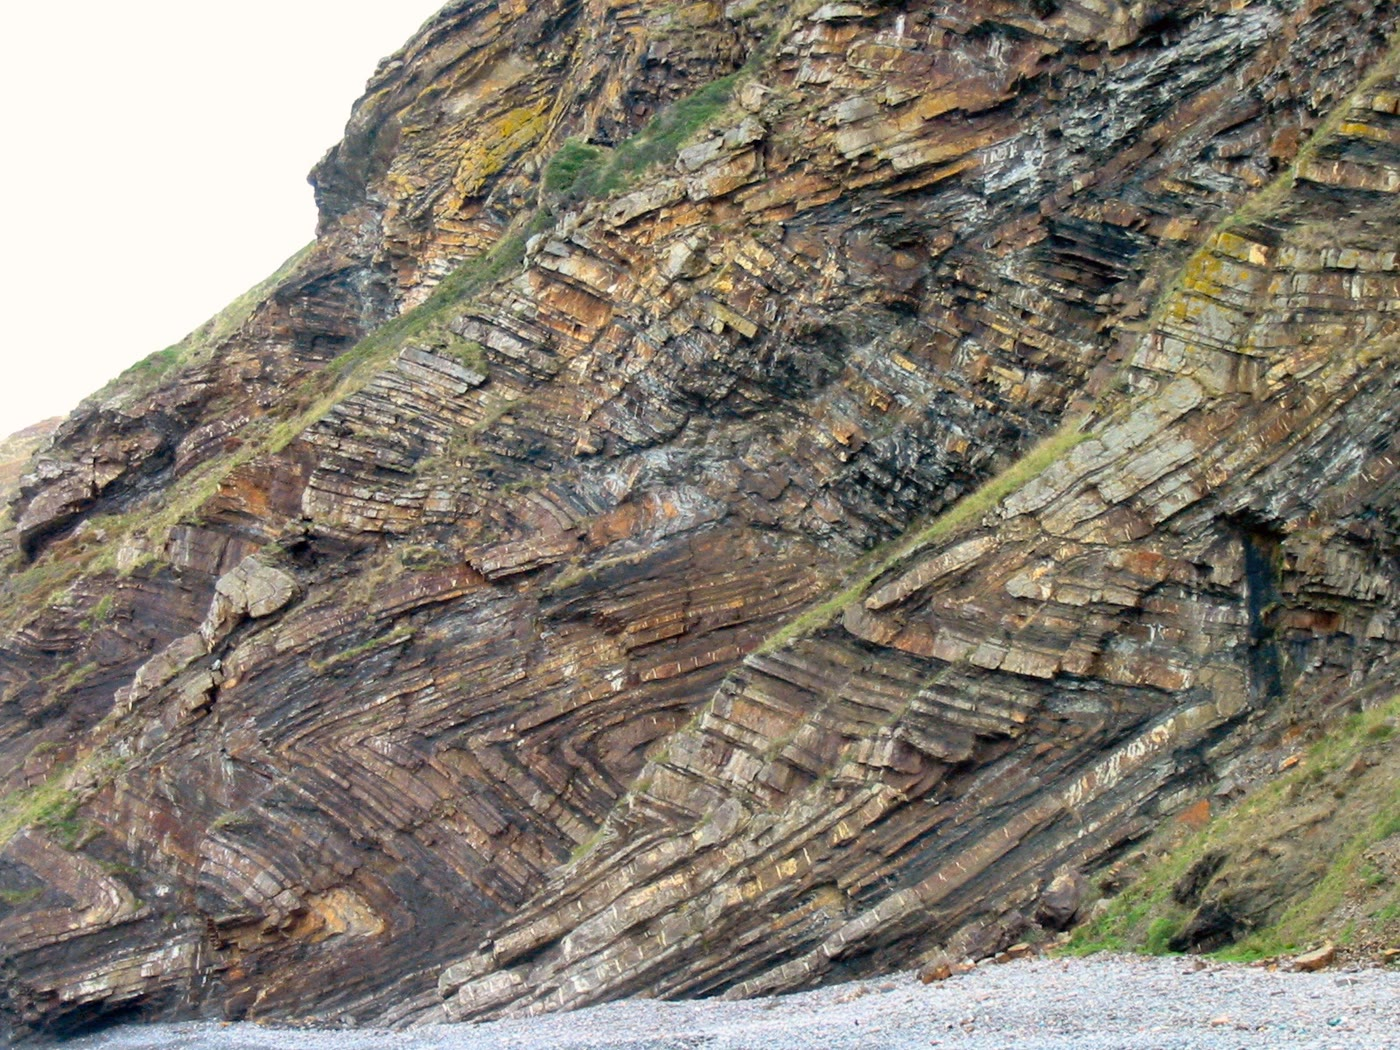
\includegraphics[width=0.78\linewidth]{images/book3/b1-chevron-folds-millook.jpg}
\par\smallskip{\small Capas plegadas de arenisca y lutita en los acantilados de Millook, en el norte de Cornualles: \omterm{def:b1:geological-maps:fold}{pliegues} en
chevrón con \omterm{def:b1:faults-folds-fabrics:fold-elements}{flancos} casi rectos y \omterm{def:b1:faults-folds-fabrics:fold-elements}{charnelas} agudas, con sus \omterm{def:b1:faults-folds-fabrics:fold-elements}{planos axiales} casi verticales. Fotografía: Smalljim, CC~BY~3.0
(Wikimedia Commons).}
\label{fig:b1:faults-folds-fabrics:chevrons}
\end{omfigure}
% ledger: commons:millook

\section{Fábricas}\label{sec:b1:faults-folds-fabrics:fabrics}

Una roca deformada suele estar deformada en todo su volumen, no solo en unas pocas superficies: sus granos se aplastan, giran
o recrecen con una orientación común, lo que le da una fábrica. Una fábrica planar hace que la roca se separe en láminas; una
fábrica lineal hace que se rompa en varillas.

\begin{definition}[Foliación, esquistosidad, clivaje pizarroso, clivaje axial-plano]\label{def:b1:faults-folds-fabrics:foliation}
Una \emph{foliación}\index{foliación} es una fábrica planar que impregna una roca: un conjunto de superficies paralelas muy
juntas, formado por granos laminares o aplastados alineados o por capas delgadas, según las cuales la roca se separa con más
facilidad. La \emph{esquistosidad}\index{esquistosidad} es la foliación de un esquisto, formada por granos alineados más gruesos
que unos \qty{1}{mm}. Un \emph{clivaje}\index{clivaje (de una roca)} es una foliación de una roca de grano fino producida por su
deformación; el \emph{clivaje pizarroso}\index{clivaje pizarroso} es el clivaje de una pizarra, formado por silicatos laminares
demasiado pequeños para verse a simple vista, y tan juntos que la roca puede separarse casi en cualquier lugar en \omterm{def:b1:field-lab-methods-1:thin-section}{láminas
delgadas}. Un \emph{clivaje axial-plano}\index{clivaje axial-plano} es un clivaje paralelo, o casi paralelo, a los \omterm{def:b1:faults-folds-fabrics:fold-elements}{planos axiales}
de los \omterm{def:b1:geological-maps:fold}{pliegues} de las mismas rocas.
\end{definition}
% ledger: ws:fabrics

Una \omterm{def:b1:faults-folds-fabrics:foliation}{foliación} se forma aproximadamente perpendicular a la dirección de mayor acortamiento, por el giro de los granos laminares,
el crecimiento de \omterm{def:b1:rock-forming-minerals:groups}{micas} nuevas y la disolución de los granos en las caras más apretadas. El \omterm{def:b1:faults-folds-fabrics:foliation}{clivaje} de una pizarra no tiene, por
tanto, nada que ver con la estratificación del lodo: registra el apretamiento. Cuando los \omterm{def:b1:geological-maps:fold}{pliegues} y el \omterm{def:b1:faults-folds-fabrics:foliation}{clivaje} crecen con el mismo
acortamiento, el \omterm{def:b1:faults-folds-fabrics:foliation}{clivaje} yace cerca de los \omterm{def:b1:faults-folds-fabrics:fold-elements}{planos axiales} de los \omterm{def:b1:geological-maps:fold}{pliegues}, y se abanica ligeramente a través de ellos, convergiendo
o divergiendo según la resistencia de cada capa, como muestra la fotografía de abajo.
% ledger: ws:fabrics

\begin{omfigure}
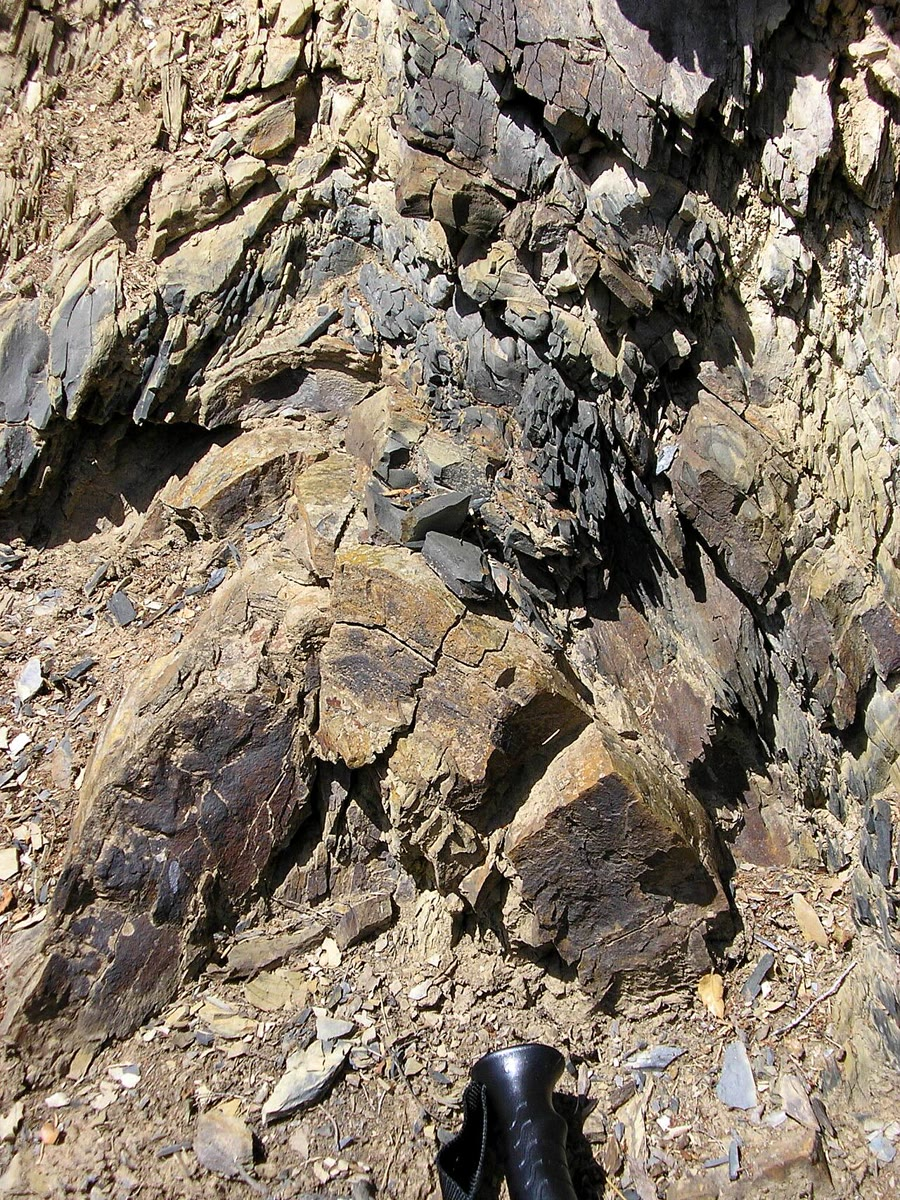
\includegraphics[height=8.2cm]{images/book3/b1-axial-planar-cleavage.jpg}
\par\smallskip{\small Un pequeño \omterm{def:b1:geological-maps:fold}{anticlinal} en una alternancia de arenisca y lutita de edad carbonífera, cerca de Potes,
Cantabria. Las capas de arenisca marrón se arquean sobre la \omterm{def:b1:faults-folds-fabrics:fold-elements}{charnela} en la parte inferior central de la imagen; en la lutita
oscura que está encima, el \omterm{def:b1:faults-folds-fabrics:foliation}{clivaje}, un conjunto de fracturas empinadas y muy juntas que cortan las capas, es axial-plano: casi
paralelo al \omterm{def:b1:faults-folds-fabrics:fold-elements}{plano axial} del \omterm{def:b1:geological-maps:fold}{pliegue}, lo atraviesa abanicándose, y el abanico cambia de una capa a otra. El mango del bastón mide
unos \qty{4}{cm} de diámetro. Fotografía: Mikenorton, CC~BY-SA~3.0 (Wikimedia Commons).}
\label{fig:b1:faults-folds-fabrics:cleavage}
\end{omfigure}
% ledger: commons:axial-cleavage

\begin{definition}[Linación, linación de intersección, linación de estiramiento]\label{def:b1:faults-folds-fabrics:lineation}
Una \emph{linación}\index{linación} es una fábrica lineal que impregna una roca, medida por su tendencia y su \omterm{def:b1:field-lab-methods-1:trend-plunge}{inmersión}. Una
\emph{linación de intersección}\index{linación de intersección} es el conjunto de rectas según las que se cortan dos fábricas
planares, como la estratificación y un \omterm{def:b1:faults-folds-fabrics:foliation}{clivaje}; una \emph{linación de estiramiento}\index{linación de estiramiento} está formada
por granos o cantos alargados según la dirección de mayor estiramiento.
\end{definition}
% ledger: ws:fabrics

\begin{proposition}[La linación de intersección de un pliegue]\label{prop:b1:faults-folds-fabrics:intersection}
En un \omterm{def:b1:faults-folds-fabrics:fold-elements}{pliegue cilíndrico} con un \omterm{def:b1:faults-folds-fabrics:foliation}{clivaje axial-plano}, la \omterm{def:b1:faults-folds-fabrics:lineation}{linación de intersección} de la estratificación y del \omterm{def:b1:faults-folds-fabrics:foliation}{clivaje} es paralela
a la \omterm{def:b1:faults-folds-fabrics:fold-elements}{línea de charnela}, en todo el \omterm{def:b1:geological-maps:fold}{pliegue}.
\end{proposition}

\begin{proof}
Cada superficie de estratificación de un \omterm{def:b1:faults-folds-fabrics:fold-elements}{pliegue cilíndrico} contiene la dirección de su eje. El \omterm{def:b1:faults-folds-fabrics:fold-elements}{plano axial} contiene las \omterm{def:b1:faults-folds-fabrics:fold-elements}{líneas
de charnela}, que son paralelas al eje, así que contiene también esa dirección, y lo mismo cualquier plano de \omterm{def:b1:faults-folds-fabrics:foliation}{clivaje} paralelo a
él. Dos planos que no son paralelos y que contienen la misma dirección se cortan según una recta de esa dirección.
\end{proof}

La proposición es el camino del geólogo de campo hacia la \omterm{def:b1:field-lab-methods-1:trend-plunge}{inmersión} de un \omterm{def:b1:geological-maps:fold}{pliegue} demasiado grande para verse entero: en cualquier
afloramiento de uno de los \omterm{def:b1:faults-folds-fabrics:fold-elements}{flancos}, las rectas según las que el \omterm{def:b1:faults-folds-fabrics:foliation}{clivaje} corta a la estratificación dan la \omterm{def:b1:faults-folds-fabrics:fold-elements}{línea de charnela}. La
estratificación y el \omterm{def:b1:faults-folds-fabrics:foliation}{clivaje} juntos dicen aún más: dónde está el \omterm{def:b1:geological-maps:fold}{pliegue}, y hacia qué lado están vueltas las capas.

\begin{definition}[Vergencia]\label{def:b1:faults-folds-fabrics:vergence}
La \emph{vergencia}\index{vergencia} de un \omterm{def:b1:geological-maps:fold}{pliegue} asimétrico es la dirección horizontal hacia la que su parte superior se ha
desplazado respecto de su parte inferior: la dirección en la que está volcado o, en un \omterm{def:b1:faults-folds-fabrics:fold-classes}{pliegue inclinado}, hacia la que se
inclina.
\end{definition}
% ledger: ws:vergence

\begin{proposition}[Estratificación y clivaje en los flancos de un pliegue]\label{prop:b1:faults-folds-fabrics:cleavage-bedding}
Considérese un \omterm{def:b1:geological-maps:fold}{pliegue} con \omterm{def:b1:faults-folds-fabrics:fold-elements}{flancos} rectos y un \omterm{def:b1:faults-folds-fabrics:foliation}{clivaje axial-plano}, en rocas que estaban en posición normal antes del plegamiento,
y en las que ambos \omterm{def:b1:faults-folds-fabrics:fold-elements}{flancos} descienden desde cada \omterm{def:b1:faults-folds-fabrics:fold-elements}{charnela} \omterm{def:b1:geological-maps:fold}{anticlinal}. Visto en el perfil:
\begin{enumerate}[label=(\alph*)]
  \item en un flanco donde la estratificación y el \omterm{def:b1:faults-folds-fabrics:foliation}{clivaje} buzan en el mismo sentido, la estratificación es la más empinada de
        las dos exactamente cuando el flanco está volcado;
  \item la rotación aguda que lleva el \omterm{def:b1:faults-folds-fabrics:foliation}{clivaje} sobre la estratificación tiene sentidos opuestos en los dos \omterm{def:b1:faults-folds-fabrics:fold-elements}{flancos} de un \omterm{def:b1:geological-maps:fold}{pliegue};
        en un flanco que no está volcado, desplaza la parte superior del \omterm{def:b1:faults-folds-fabrics:foliation}{clivaje} horizontalmente hacia la \omterm{def:b1:faults-folds-fabrics:fold-elements}{charnela} \omterm{def:b1:geological-maps:fold}{anticlinal} de la
        parte superior de ese flanco.
\end{enumerate}
\end{proposition}

\begin{proof}
Mírese a lo largo de la \omterm{def:b1:faults-folds-fabrics:fold-elements}{charnela}, con el \omterm{def:b1:faults-folds-fabrics:fold-elements}{plano axial} buzando hacia la izquierda con el ángulo
$\gamma$, $0 < \gamma \le \ang{90}$, y cuéntense los ángulos en sentido antihorario desde la horizontal apuntando a la derecha.
El \omterm{def:b1:faults-folds-fabrics:foliation}{clivaje}, paralelo al \omterm{def:b1:faults-folds-fabrics:fold-elements}{plano axial}, sube con el ángulo $\gamma$. En una \omterm{def:b1:faults-folds-fabrics:fold-elements}{charnela} \omterm{def:b1:geological-maps:fold}{anticlinal} los dos \omterm{def:b1:faults-folds-fabrics:fold-elements}{flancos} salen hacia abajo con
los ángulos $\ang{180} + \gamma - \iota/2$ (flanco~1) y $\ang{180} + \gamma + \iota/2$ (flanco~2), a cada lado del \omterm{def:b1:faults-folds-fabrics:fold-elements}{plano axial},
con $\iota/2 \le \gamma$ porque ambos descienden; cada flanco de una serie de \omterm{def:b1:geological-maps:fold}{pliegues} es uno de estos dos para el \omterm{def:b1:geological-maps:fold}{anticlinal}
de su parte superior. Las rocas se hacen más jóvenes hacia fuera, alejándose del núcleo del \omterm{def:b1:geological-maps:fold}{anticlinal}, a lo largo de la normal
al flanco que apunta lejos del \omterm{def:b1:faults-folds-fabrics:fold-elements}{plano axial}.

El flanco~1 baja hacia la izquierda: buza hacia la izquierda con $\gamma - \iota/2$, menos empinado que el \omterm{def:b1:faults-folds-fabrics:foliation}{clivaje}. Su normal
hacia fuera, en $\ang{90} + \gamma -
\iota/2$, apunta hacia arriba: está en posición normal. Subiendo, forma con el \omterm{def:b1:faults-folds-fabrics:foliation}{clivaje} el
ángulo $\gamma - \iota/2$, así que la rotación aguda del \omterm{def:b1:faults-folds-fabrics:foliation}{clivaje} a la estratificación es en el sentido de las agujas del reloj,
a través de $\iota/2$: la parte superior del \omterm{def:b1:faults-folds-fabrics:foliation}{clivaje} se desplaza hacia la derecha, donde está la \omterm{def:b1:faults-folds-fabrics:fold-elements}{charnela}, ya que el flanco sale
de la \omterm{def:b1:faults-folds-fabrics:fold-elements}{charnela} hacia la izquierda.

El flanco~2 forma con la horizontal, subiendo, el ángulo $\gamma + \iota/2$. Si $\gamma + \iota/2 > \ang{90}$, baja hacia la
derecha y buza hacia la derecha, en sentido opuesto al \omterm{def:b1:faults-folds-fabrics:foliation}{clivaje}; su normal hacia fuera, en $\ang{270} + \gamma +
\iota/2$, tiene la
componente hacia arriba $-\cos(\gamma + \iota/2) > 0$: está en posición normal. Si $\gamma + \iota/2 < \ang{90}$, baja hacia la
izquierda, buzando hacia la izquierda con $\gamma + \iota/2$, más empinado que el \omterm{def:b1:faults-folds-fabrics:foliation}{clivaje}, y la misma componente es negativa: el
flanco está volcado. En ambos casos la rotación aguda del \omterm{def:b1:faults-folds-fabrics:foliation}{clivaje} a la estratificación es en sentido antihorario, a través de
$\iota/2$, y desplaza la parte superior del \omterm{def:b1:faults-folds-fabrics:foliation}{clivaje} hacia la izquierda; cuando el flanco está en posición normal sale de la \omterm{def:b1:faults-folds-fabrics:fold-elements}{charnela}
hacia la derecha, así que la \omterm{def:b1:faults-folds-fabrics:fold-elements}{charnela} está a la izquierda. Los \omterm{def:b1:faults-folds-fabrics:fold-elements}{flancos} que buzan en el mismo sentido que el \omterm{def:b1:faults-folds-fabrics:foliation}{clivaje} son así el
flanco~1, menos empinado, y un flanco~2 volcado, más empinado, que es (a); los sentidos son en el sentido de las agujas del reloj
en el flanco~1 y en sentido antihorario en el flanco~2, que es (b).
\end{proof}

El sentido de la rotación cambia, así, en cada \omterm{def:b1:faults-folds-fabrics:fold-elements}{charnela}, \omterm{def:b1:geological-maps:fold}{anticlinal} o \omterm{def:b1:geological-maps:fold}{sinclinal}. Un geólogo que lo anota a lo largo de un recorrido
encuentra las \omterm{def:b1:faults-folds-fabrics:fold-elements}{charnelas} de \omterm{def:b1:geological-maps:fold}{pliegues} demasiado grandes para verse en un solo afloramiento donde cambia el sentido, y los \omterm{def:b1:faults-folds-fabrics:fold-elements}{flancos}
volcados donde la estratificación es más empinada que el \omterm{def:b1:faults-folds-fabrics:foliation}{clivaje}; la palabra \omterm{def:b1:faults-folds-fabrics:vergence}{vergencia} se usa también para este sentido de
rotación, y las inversiones de la \omterm{def:b1:faults-folds-fabrics:vergence}{vergencia} de \omterm{def:b1:geological-maps:fold}{pliegues} menores se cartografían del mismo modo para encontrar las \omterm{def:b1:faults-folds-fabrics:fold-elements}{charnelas} de
\omterm{def:b1:geological-maps:fold}{pliegues} mayores: los pequeños \omterm{def:b1:geological-maps:fold}{pliegues} de los dos \omterm{def:b1:faults-folds-fabrics:fold-elements}{flancos} de uno grande tienen asimetrías opuestas, y su traza axial pasa entre ellos.
% ledger: ws:vergence, ws:fold-elements

\begin{omfigure}
\begin{tikzpicture}[>={Stealth[length=5pt]}, font=\small]
% a train of chevron folds seen along the hinge (north into the page, east to the right):
% axial planes dipping 60 deg to the west, interlimb angle 40 deg; long limbs dip 40 deg W
% (the right way up), short limbs 80 deg W (overturned). Short limb: from an anticline hinge H_k,
% length s along 260 deg to the syncline hinge S_k; long limb back up along 40 deg to H_{k+1},
% so that all anticline hinges are level, a wavelength w apart.
% Five bedding surfaces, repeated along the axial direction (similar folds); cleavage parallel to it.
\def\s{2.6}
\pgfmathsetmacro{\sx}{\s*cos(260)}\pgfmathsetmacro{\sy}{\s*sin(260)}
\pgfmathsetmacro{\w}{\sx - \sy/tan(40)}
\pgfmathsetmacro{\hx}{0.62*cos(60)}\pgfmathsetmacro{\hy}{0.62*sin(60)}
\newcommand{\surface}[1]{%
  (-\w+#1*\hx, #1*\hy) \foreach \k in {-1,0,1,2,3} { -- ({\k*\w+\sx+#1*\hx}, {\sy+#1*\hy}) -- ({(\k+1)*\w+#1*\hx}, {#1*\hy}) }}
\begin{scope}
  \clip (0.35,-3.3) rectangle (10.0,2.95);
  \begin{scope}
    \clip \surface{0} -- (12,6) -- (-4,6) -- cycle;
    \clip \surface{4} -- (12,-6) -- (-4,-6) -- cycle;
    \fill[omLithSand!45] (-4,-6) rectangle (12,6);
    \fill[omLithShale!40] \surface{2} -- (12,6) -- (-4,6) -- cycle;
    \fill[omLithSand!45] \surface{3} -- (12,6) -- (-4,6) -- cycle;
    \foreach \c in {-8.0,-7.78,...,13.0} {
      \draw[omDef!85, line width=0.35pt] ({\c-6*cot(60)},-6) -- ({\c+6*cot(60)},6);
    }
  \end{scope}
  \foreach \j in {0,1,2,3,4} { \draw[line width=0.75pt, line join=round] \surface{\j}; }
\end{scope}
% axial traces through the anticline hinges, and labels
\foreach \k in {1,2,3} {
  \draw[omThm, dashed, line width=0.6pt] ({\k*\w-0.5*cos(60)},{-0.5*sin(60)}) -- ({\k*\w+3.6*cos(60)},{3.6*sin(60)});
  \node[omThm, font=\scriptsize, anchor=south] at ({\k*\w+3.6*cos(60)},{3.6*sin(60)}) {anticlinal};
}
\foreach \k in {1,2,3} { \node[omThm, font=\scriptsize, anchor=north] at ({\k*\w+\sx},{\sy-0.15}) {sinclinal}; }
\end{tikzpicture}
\par\smallskip{\small Un tren de \omterm{def:b1:geological-maps:fold}{pliegues} en chevrón volcados hacia la derecha, en perfil, con un \omterm{def:b1:faults-folds-fabrics:foliation}{clivaje axial-plano} (líneas azules
finas), dibujado a escala: \omterm{def:b1:faults-folds-fabrics:fold-elements}{planos axiales} que buzan \ang{60} hacia la izquierda, \omterm{def:b1:faults-folds-fabrics:fold-elements}{ángulo entre flancos} \ang{40}. Los \omterm{def:b1:faults-folds-fabrics:fold-elements}{flancos}
largos buzan \ang{40} hacia la izquierda, menos empinados que el \omterm{def:b1:faults-folds-fabrics:foliation}{clivaje}, y están en posición normal; los \omterm{def:b1:faults-folds-fabrics:fold-elements}{flancos} cortos buzan
\ang{80} hacia la izquierda, más empinados que el \omterm{def:b1:faults-folds-fabrics:foliation}{clivaje}, y están volcados. Girar el \omterm{def:b1:faults-folds-fabrics:foliation}{clivaje} sobre la estratificación por el
ángulo agudo es en el sentido de las agujas del reloj en todos los \omterm{def:b1:faults-folds-fabrics:fold-elements}{flancos} largos y en sentido antihorario en todos los \omterm{def:b1:faults-folds-fabrics:fold-elements}{flancos}
cortos. Los \omterm{def:b1:geological-maps:fold}{pliegues} vergen hacia la derecha.}
\label{fig:b1:faults-folds-fabrics:vergence}
\end{omfigure}

\section{Microestructuras}\label{sec:b1:faults-folds-fabrics:micro}

Al microscopio, la deformación de una roca se manifiesta en sus granos. Un grano de cuarzo doblado por el lento deslizamiento de su
red cristalina ya no se extingue de golpe entre polarizadores cruzados: al girar la platina, una banda oscura lo recorre, porque
sus partes apuntan en direcciones ligeramente distintas. Esta extinción ondulante (\cref{ch:b1:optical-mineralogy}) se hace más
fuerte al acercarse a una zona de cizalla, porque los defectos se acumulan en la red cristalina. Donde hay agua, los granos se
disuelven en las caras donde están más apretados, y la materia disuelta se deposita donde el esfuerzo es menor, o se lleva: esta
solución por presión acorta las rocas a baja temperatura y produce muchos \omterm{def:b1:faults-folds-fabrics:foliation}{clivajes}. A temperatura más alta, los granos deformados
se sustituyen, mientras la deformación continúa, por granos nuevos, más pequeños y sin deformar, primero a lo largo de los antiguos
bordes de grano: recristalización dinámica, que reduce el tamaño de grano y produce las \omterm{def:b1:faults-folds-fabrics:fault-rocks}{milonitas}. Las formas de los granos
deformados y de los \omterm{def:b1:rock-forming-minerals:mineral}{minerales} que crecen en sus sombras indican también hacia dónde se movió una zona de cizalla; estos indicadores
del sentido de cizalla, y los mecanismos mismos, pertenecen al volumen del año~3.
% ledger: ws:microstructures, ws:fabrics

\section{Ejercicios}

\begin{exercise}[$\star$]\label{exo:b1:faults-folds-fabrics:1}
Nómbrese cada falla según el \omterm{def:b1:faults-folds-fabrics:fault-elements}{cabeceo} de su \omterm{def:b1:faults-folds-fabrics:fault-elements}{vector de deslizamiento}, con la falla buzando \ang{60}: (a) $r = \ang{-90}$; (b) $r = \ang{85}$;
(c) $r = 0$; (d) $r = \ang{180}$; (e) $r = \ang{-40}$. (f) ¿Cómo se llamaría (b) si su \omterm{def:b1:geological-maps:attitude}{buzamiento} fuera \ang{25}?
% ledger: ar:rake, usgs:fault-types
\end{exercise}

\begin{exercise}[$\star$]\label{exo:b1:faults-folds-fabrics:2}
Una \omterm{def:b1:faults-folds-fabrics:fault-types}{falla normal} buza \ang{55}; su deslizamiento es puramente de \omterm{def:b1:geological-maps:attitude}{buzamiento}, con un \omterm{def:b1:faults-folds-fabrics:fault-elements}{deslizamiento neto} de \qty{300}{m}.
Calcúlense su salto y su \omterm{def:b1:cross-sections:throw}{salto horizontal}.
\end{exercise}

\begin{exercise}[$\star$]\label{exo:b1:faults-folds-fabrics:3}
Dese el \omterm{def:b1:faults-folds-fabrics:fold-elements}{ángulo entre flancos} y la clase de cada \omterm{def:b1:faults-folds-fabrics:fold-classes}{pliegue erguido}, cuyos \omterm{def:b1:faults-folds-fabrics:fold-elements}{flancos} buzan en sentidos opuestos: (a) \omterm{def:b1:faults-folds-fabrics:fold-elements}{flancos} que buzan
\ang{35} y \ang{35}; (b) \ang{70} y \ang{75}; (c) \ang{85} y \ang{88}.
% ledger: ws:fold-classes
\end{exercise}

\begin{exercise}[$\star$]\label{exo:b1:faults-folds-fabrics:4}
Una arenisca tiene un \omterm{def:b1:stress-strain-rheology:coulomb}{ángulo de fricción interna} de \ang{35}. Según la teoría de Anderson, ¿con qué ángulos buzan sus \omterm{def:b1:faults-folds-fabrics:fault-types}{fallas
normales} y sus \omterm{def:b1:faults-folds-fabrics:fault-types}{cabalgamientos}? ¿Qué ángulo forman entre sí dos \omterm{def:b1:faults-folds-fabrics:fault-types}{fallas de desgarre} conjugadas?
\end{exercise}

\begin{exercise}[$\star\star$]\label{exo:b1:faults-folds-fabrics:5}
Una falla tiene la \omterm{def:b1:geological-maps:attitude}{actitud} $090/50$, y sobre ella estrías de \omterm{def:b1:faults-folds-fabrics:fault-elements}{cabeceo} \ang{-30}; el \omterm{def:b1:faults-folds-fabrics:fault-elements}{deslizamiento neto} es \qty{400}{m}. (a) Calcúlense
las componentes de desgarre y de \omterm{def:b1:geological-maps:attitude}{buzamiento}, el salto y el \omterm{def:b1:cross-sections:throw}{salto horizontal}. (b) Escríbase el \omterm{def:b1:faults-folds-fabrics:fault-elements}{vector de deslizamiento} en
componentes hacia el este, el norte y arriba, y dense su tendencia e \omterm{def:b1:field-lab-methods-1:trend-plunge}{inmersión}. (c) Nómbrese la falla.
\end{exercise}

\begin{exercise}[$\star\star$]\label{exo:b1:faults-folds-fabrics:6}
Dos \omterm{def:b1:faults-folds-fabrics:fault-types}{fallas de desgarre} verticales de la misma edad tienen \omterm{def:b1:geological-maps:attitude}{rumbos} $020$ y $080$. (a) Según Anderson, dense las direcciones de
$\sigma_1$, $\sigma_2$ y $\sigma_3$, y el \omterm{def:b1:stress-strain-rheology:coulomb}{ángulo de fricción interna} de la roca. (b) ¿Cuál falla es \omterm{def:b1:faults-folds-fabrics:fault-types}{dextral} y cuál \omterm{def:b1:faults-folds-fabrics:fault-types}{sinistral}?
Razónese a partir del acortamiento según $\sigma_1$.
\end{exercise}

\begin{exercise}[$\star\star$]\label{exo:b1:faults-folds-fabrics:7}
Los dos \omterm{def:b1:faults-folds-fabrics:fold-elements}{flancos} de un \omterm{def:b1:faults-folds-fabrics:fold-elements}{pliegue cilíndrico} tienen las \omterm{def:b1:geological-maps:attitude}{actitudes} $120/40$ y $260/30$. Con
\cref{prop:b1:faults-folds-fabrics:hinge}, hállense la tendencia y la \omterm{def:b1:field-lab-methods-1:trend-plunge}{inmersión} de su \omterm{def:b1:faults-folds-fabrics:fold-elements}{línea de charnela}, su \omterm{def:b1:faults-folds-fabrics:fold-elements}{ángulo entre flancos} y su clase.
\end{exercise}

\begin{exercise}[$\star\star$]\label{exo:b1:faults-folds-fabrics:8}
En un afloramiento, la estratificación tiene la \omterm{def:b1:geological-maps:attitude}{actitud} $040/30$ y un \omterm{def:b1:faults-folds-fabrics:foliation}{clivaje axial-plano} la \omterm{def:b1:geological-maps:attitude}{actitud} $160/80$. Hállense la tendencia y la
\omterm{def:b1:field-lab-methods-1:trend-plunge}{inmersión} de la \omterm{def:b1:faults-folds-fabrics:lineation}{linación de intersección}. ¿Qué dice sobre el \omterm{def:b1:geological-maps:fold}{pliegue}?
\end{exercise}

\begin{exercise}[$\star\star$]\label{exo:b1:faults-folds-fabrics:9}
Una falla vertical tiene \omterm{def:b1:geological-maps:attitude}{rumbo} este--oeste. Un dique vertical de \omterm{def:b1:geological-maps:attitude}{rumbo} norte--sur la atraviesa; al norte de la falla, el dique aparece
\qty{350}{m} al este de donde está al sur de la falla. (a) ¿Es la falla \omterm{def:b1:faults-folds-fabrics:fault-types}{dextral} o \omterm{def:b1:faults-folds-fabrics:fault-types}{sinistral}? (b) Si las estrías son horizontales,
¿cuál es el \omterm{def:b1:faults-folds-fabrics:fault-elements}{deslizamiento neto}? (c) Si en cambio se inclinan \ang{20} hacia el este, ¿cuáles son el \omterm{def:b1:faults-folds-fabrics:fault-elements}{deslizamiento neto} y la componente
vertical del deslizamiento, y qué bloque bajó?
\end{exercise}

\begin{exercise}[$\star\star\star$]\label{exo:b1:faults-folds-fabrics:10}
Una falla sin \omterm{def:b1:stress-strain-rheology:coulomb}{cohesión} y con coeficiente de fricción $\mu$ forma el ángulo $\theta$ con $\sigma_1$. (a) Demuéstrese que desliza
cuando los \omterm{def:b1:stress-strain-rheology:principal}{esfuerzos principales} efectivos alcanzan el cociente
\[
  \frac{\sigma_1'}{\sigma_3'} = \frac{1 + \mu\cot\theta}{1 - \mu\tan\theta} .
\]
(b) Con $\mu = 0.6$ y $\sigma_1$ vertical, calcúlese el cociente para \omterm{def:b1:faults-folds-fabrics:fault-types}{fallas normales} que buzan \ang{60}, \ang{45} y \ang{35}.
(c) Demuéstrese que una \omterm{def:b1:faults-folds-fabrics:fault-types}{falla normal} que buza menos que cierto ángulo no puede deslizar nunca, y calcúlese ese ángulo. (d) Para
$\mu = 0.6$ y $\mu = 0.85$, dense los \omterm{def:b1:geological-maps:attitude}{buzamientos} de las \omterm{def:b1:faults-folds-fabrics:fault-types}{fallas normales} y de \omterm{def:b1:faults-folds-fabrics:fault-types}{cabalgamiento} de mejor orientación.
\end{exercise}

\begin{exercise}[$\star\star\star$]\label{exo:b1:faults-folds-fabrics:11}
A lo largo de un recorrido de este a oeste, atravesando \omterm{def:b1:geological-maps:fold}{pliegues} en chevrón cuyas \omterm{def:b1:faults-folds-fabrics:fold-elements}{charnelas} tienen tendencia norte, un \omterm{def:b1:faults-folds-fabrics:foliation}{clivaje
axial-plano} buza \ang{60} hacia el oeste en todas partes. La estratificación buza \ang{40} O en la estación A, \ang{80} O en la
estación B y \ang{40} O en la estación C, de oeste a este, en rocas que estaban en posición normal antes del plegamiento. (a) ¿Qué
estación está en un flanco volcado? (b) ¿En qué sentido gira el \omterm{def:b1:faults-folds-fabrics:foliation}{clivaje} sobre la estratificación en cada estación, mirando al
norte? (c) ¿Dónde están las \omterm{def:b1:faults-folds-fabrics:fold-elements}{charnelas}, y cuáles son \omterm{def:b1:geological-maps:fold}{anticlinales}? (d) Calcúlense el \omterm{def:b1:faults-folds-fabrics:fold-elements}{ángulo entre flancos} y la \omterm{def:b1:geological-maps:attitude}{actitud} de los
\omterm{def:b1:faults-folds-fabrics:fold-elements}{planos axiales}, y dígase hacia qué lado vergen los \omterm{def:b1:geological-maps:fold}{pliegues}.
\end{exercise}

\begin{exercise}[$\star\star\star$]\label{exo:b1:faults-folds-fabrics:12}
Un estrato de longitud $L_0$ se pliega en un tren de \omterm{def:b1:geological-maps:fold}{pliegues} en chevrón simétricos de \omterm{def:b1:faults-folds-fabrics:fold-elements}{ángulo entre flancos} $\iota$, sin cambiar
su longitud. (a) Demuéstrese que su longitud medida a través de los \omterm{def:b1:geological-maps:fold}{pliegues} pasa a ser $L_0\sin(\iota/2)$. (b) ¿Qué acortamiento
representan \omterm{def:b1:geological-maps:fold}{pliegues} en chevrón de \omterm{def:b1:faults-folds-fabrics:fold-elements}{ángulo entre flancos} \ang{60}? (c) ¿Qué \omterm{def:b1:faults-folds-fabrics:fold-elements}{ángulo entre flancos} corresponde a un acortamiento de
\qty{30}{\percent}? (d) Un tren de \omterm{def:b1:faults-folds-fabrics:fold-classes}{pliegues erguidos} con \omterm{def:b1:faults-folds-fabrics:fold-elements}{flancos} que buzan \ang{12}: ¿qué acortamiento?
\end{exercise}

\section{Problema: las estructuras de las Varden Hills, medidas}

\begin{problem}[{Problema de fin de semana --- el anticlinal y la falla normal de las Varden Hills, a partir de las actitudes de sus
planos y del deslizamiento sobre la falla}]
\label{pb:b1:faults-folds-fabrics:1}
% values: calc/ch17.py; region: figdata/shared/region.py (limbs, plunge, fault)
Las Varden Hills están plegadas en un \omterm{def:b1:geological-maps:fold}{anticlinal}, cuyo eje corre de norte a sur en $x = \qty{3.5}{km}$, y en un \omterm{def:b1:geological-maps:fold}{sinclinal} situado
\qty{4}{km} al este de él; ambos tienen \omterm{def:b1:faults-folds-fabrics:fold-elements}{flancos} planos. Un levantamiento de campo midió la estratificación en el flanco este del
\omterm{def:b1:geological-maps:fold}{anticlinal} como $080.7/12.2$, y en su flanco oeste como $279.3/12.2$. La cobertera está cortada por una \omterm{def:b1:faults-folds-fabrics:fault-types}{falla normal} de \omterm{def:b1:geological-maps:attitude}{actitud}
$120/60$, cuyo \omterm{def:b1:faults-folds-fabrics:fault-elements}{bloque superior} bajó según el \omterm{def:b1:geological-maps:attitude}{buzamiento}, con un salto de \qty{200}{m}. Dense los ángulos con una precisión de
\ang{0.1} y las longitudes con una precisión de \qty{0.1}{m}.

\medskip
\noindent\textbf{Parte I --- Los flancos.}
\begin{enumerate}
  \item Escríbanse las normales unitarias hacia arriba $\mathbf n_1$ (flanco este) y $\mathbf n_2$ (flanco oeste) en componentes
        hacia el este, el norte y arriba.
  \item Calcúlense $\mathbf n_1\cdot\mathbf n_2$ y el ángulo entre las normales.
  \item Dedúzcase el \omterm{def:b1:faults-folds-fabrics:fold-elements}{ángulo entre flancos} del \omterm{def:b1:geological-maps:fold}{anticlinal}.
  \item Clasifíquese el \omterm{def:b1:geological-maps:fold}{anticlinal} por su \omterm{def:b1:faults-folds-fabrics:fold-elements}{ángulo entre flancos}.
  \item Los dos \omterm{def:b1:faults-folds-fabrics:fold-elements}{flancos} buzan \ang{12.2}. ¿Por qué el \omterm{def:b1:faults-folds-fabrics:fold-elements}{ángulo entre flancos} no es exactamente
        $\ang{180} - 2\times\ang{12.2}$? Calcúlese el \omterm{def:b1:cross-sections:apparent-dip}{buzamiento aparente} de cualquiera de los \omterm{def:b1:faults-folds-fabrics:fold-elements}{flancos} en una sección vertical
        este--oeste.
  \item El \omterm{def:b1:geological-maps:fold}{sinclinal} comparte el flanco este del \omterm{def:b1:geological-maps:fold}{anticlinal}, y su propio flanco este es paralelo al flanco oeste del \omterm{def:b1:geological-maps:fold}{anticlinal}.
        ¿Cuál es su \omterm{def:b1:faults-folds-fabrics:fold-elements}{ángulo entre flancos}?
\end{enumerate}

\medskip
\noindent\textbf{Parte II --- La línea de charnela y el plano axial.}
\begin{enumerate}[resume]
  \item Calcúlese $\mathbf n_1\times\mathbf n_2$, y la tendencia y la \omterm{def:b1:field-lab-methods-1:trend-plunge}{inmersión} de la \omterm{def:b1:faults-folds-fabrics:fold-elements}{línea de charnela}.
  \item Dése la \omterm{def:b1:geological-maps:attitude}{actitud} del \omterm{def:b1:faults-folds-fabrics:fold-elements}{plano axial}. ¿Es el \omterm{def:b1:geological-maps:fold}{anticlinal} erguido, inclinado o recumbente?
  \item Dése la descripción completa del \omterm{def:b1:geological-maps:fold}{pliegue}: estrechez, \omterm{def:b1:geological-maps:attitude}{actitud} del \omterm{def:b1:faults-folds-fabrics:fold-elements}{plano axial}, \omterm{def:b1:field-lab-methods-1:trend-plunge}{inmersión}.
  \item En el \omterm{def:b1:geological-maps:geological-map}{mapa geológico} de \cref{ch:b1:geological-maps}, ¿hacia qué lado se cierran los afloramientos del \omterm{def:b1:geological-maps:fold}{anticlinal}, y qué
        aflora en su núcleo?
  \item La lutita de la cobertera tiene un \omterm{def:b1:faults-folds-fabrics:foliation}{clivaje axial-plano}. Dése su \omterm{def:b1:geological-maps:attitude}{actitud}, y la tendencia y la \omterm{def:b1:field-lab-methods-1:trend-plunge}{inmersión} de su \omterm{def:b1:faults-folds-fabrics:lineation}{linación de
        intersección} en el flanco este.
  \item En el flanco este, ¿en qué sentido gira el \omterm{def:b1:faults-folds-fabrics:foliation}{clivaje} sobre la estratificación, visto mirando al norte, y en qué lado está la
        \omterm{def:b1:faults-folds-fabrics:fold-elements}{charnela} del \omterm{def:b1:geological-maps:fold}{anticlinal}?
\end{enumerate}

\medskip
\noindent\textbf{Parte III --- La falla y los esfuerzos.}
\begin{enumerate}[resume]
  \item Dése el \omterm{def:b1:geological-maps:attitude}{rumbo} de la falla por la regla de la mano derecha, e indique en qué lado de su traza yace el \omterm{def:b1:faults-folds-fabrics:fault-elements}{bloque superior}.
  \item Según Anderson, ¿qué esfuerzo principal era vertical cuando se formó la falla?
  \item Dense las direcciones de los dos \omterm{def:b1:stress-strain-rheology:principal}{esfuerzos principales} horizontales.
  \item ¿Qué \omterm{def:b1:stress-strain-rheology:coulomb}{ángulo de fricción interna} implica el \omterm{def:b1:geological-maps:attitude}{buzamiento}? ¿Qué \omterm{def:b1:stress-strain-rheology:coulomb}{coeficiente de fricción interna}?
  \item Dese la \omterm{def:b1:geological-maps:attitude}{actitud} del conjunto conjugado de fallas que podrían haber formado los mismos esfuerzos, y el ángulo entre los dos conjuntos.
  \item ¿Estaría la falla bien orientada para deslizar de nuevo bajo el mismo régimen, con la fricción de Byerlee de 0.85?
\end{enumerate}

\medskip
\noindent\textbf{Parte IV --- El deslizamiento.}
\begin{enumerate}[resume]
  \item Dése el \omterm{def:b1:faults-folds-fabrics:fault-elements}{cabeceo} del \omterm{def:b1:faults-folds-fabrics:fault-elements}{vector de deslizamiento}, y su tendencia e \omterm{def:b1:field-lab-methods-1:trend-plunge}{inmersión}.
  \item Escríbase el vector unitario del deslizamiento en componentes hacia el este, el norte y arriba.
  \item Calcúlese el \omterm{def:b1:cross-sections:throw}{salto horizontal} de la falla.
  \item Calcúlense las componentes hacia el este y hacia el norte del desplazamiento horizontal del \omterm{def:b1:faults-folds-fabrics:fault-elements}{bloque superior}.
  \item Compruébese que el \omterm{def:b1:faults-folds-fabrics:fault-elements}{deslizamiento neto} $L$, el salto $h$ y el \omterm{def:b1:cross-sections:throw}{salto horizontal} $e$ cumplen $L^2 = h^2 + e^2$, y explíquese por qué.
  \item Redondeando al metro, ¿cuál es el \omterm{def:b1:faults-folds-fabrics:fault-elements}{deslizamiento neto} de la falla de Varden?
\end{enumerate}
\end{problem}
